\documentclass[journal,12pt,twocolumn]{IEEEtran}
\usepackage{setspace}
\usepackage{gensymb}
\usepackage{caption}
%\usepackage{multirow}
%\usepackage{multicolumn}
%\usepackage{subcaption}
%\doublespacing
\singlespacing
\usepackage{csvsimple}
\usepackage{amsmath}
\usepackage{multicol}
%\usepackage{enumerate}
\usepackage{amssymb}
%\usepackage{graphicx}
\usepackage{newfloat}
%\usepackage{syntax}
\usepackage{listings}
\usepackage{iithtlc}
\usepackage{color}
\usepackage{tikz}
\usetikzlibrary{shapes,arrows}



%\usepackage{graphicx}
%\usepackage{amssymb}
%\usepackage{relsize}
%\usepackage[cmex10]{amsmath}
%\usepackage{mathtools}
%\usepackage{amsthm}
%\interdisplaylinepenalty=2500
%\savesymbol{iint}
%\usepackage{txfonts}
%\restoresymbol{TXF}{iint}
%\usepackage{wasysym}
\usepackage{amsthm}
\usepackage{mathrsfs}
\usepackage{txfonts}
\usepackage{stfloats}
\usepackage{cite}
\usepackage{cases}
\usepackage{mathtools}
\usepackage{caption}
\usepackage{enumerate}	
\usepackage{enumitem}
\usepackage{amsmath}
%\usepackage{xtab}
\usepackage{longtable}
\usepackage{multirow}
%\usepackage{algorithm}
%\usepackage{algpseudocode}
\usepackage{enumitem}
\usepackage{chngcntr}
\usepackage{mathtools}
\usepackage{hyperref}
%\usepackage[framemethod=tikz]{mdframed}
\usepackage{listings}
    %\usepackage[latin1]{inputenc}                                 %%
    \usepackage{color}                                            %%
    \usepackage{array}                                            %%
    \usepackage{longtable}                                        %%
    \usepackage{calc}                                             %%
    \usepackage{multirow}                                         %%
    \usepackage{hhline}                                           %%
    \usepackage{ifthen}                                           %%
  %optionally (for landscape tables embedded in another document): %%
    \usepackage{lscape}     


\usepackage{url}
\def\UrlBreaks{\do\/\do-}


%\usepackage{stmaryrd}


%\usepackage{wasysym}
%\newcounter{MYtempeqncnt}
\DeclareMathOperator*{\Res}{Res}
%\renewcommand{\baselinestretch}{2}
\renewcommand\thesection{\arabic{section}}
\renewcommand\thesubsection{\thesection.\arabic{subsection}}
\renewcommand\thesubsubsection{\thesubsection.\arabic{subsubsection}}

\renewcommand\thesectiondis{\arabic{section}}
\renewcommand\thesubsectiondis{\thesectiondis.\arabic{subsection}}
\renewcommand\thesubsubsectiondis{\thesubsectiondis.\arabic{subsubsection}}

% correct bad hyphenation here
\hyphenation{op-tical net-works semi-conduc-tor}

%\lstset{
%language=C,
%frame=single, 
%breaklines=true
%}

%\lstset{
	%%basicstyle=\small\ttfamily\bfseries,
	%%numberstyle=\small\ttfamily,
	%language=Octave,
	%backgroundcolor=\color{white},
	%%frame=single,
	%%keywordstyle=\bfseries,
	%%breaklines=true,
	%%showstringspaces=false,
	%%xleftmargin=-10mm,
	%%aboveskip=-1mm,
	%%belowskip=0mm
%}

%\surroundwithmdframed[width=\columnwidth]{lstlisting}
\def\inputGnumericTable{}                                 %%
\lstset{
%language=C,
frame=single, 
breaklines=true,
columns=fullflexible
}
 

\begin{document}
%
\tikzstyle{block} = [rectangle, draw,
    text width=3em, text centered, minimum height=3em]
\tikzstyle{sum} = [draw, circle, node distance=3cm]
\tikzstyle{input} = [coordinate]
\tikzstyle{output} = [coordinate]
\tikzstyle{pinstyle} = [pin edge={to-,thin,black}]

\theoremstyle{definition}
\newtheorem{theorem}{Theorem}[section]
\newtheorem{problem}{Problem}
\newtheorem{proposition}{Proposition}[section]
\newtheorem{lemma}{Lemma}[section]
\newtheorem{corollary}[theorem]{Corollary}
\newtheorem{example}{Example}[section]
\newtheorem{definition}{Definition}[section]
%\newtheorem{algorithm}{Algorithm}[section]
%\newtheorem{cor}{Corollary}
\newcommand{\BEQA}{\begin{eqnarray}}
\newcommand{\EEQA}{\end{eqnarray}}
\newcommand{\define}{\stackrel{\triangle}{=}}

\bibliographystyle{IEEEtran}
%\bibliographystyle{ieeetr}

\providecommand{\nCr}[2]{\,^{#1}C_{#2}} % nCr
\providecommand{\nPr}[2]{\,^{#1}P_{#2}} % nPr
\providecommand{\mbf}{\mathbf}
\providecommand{\pr}[1]{\ensuremath{\Pr\left(#1\right)}}
\providecommand{\qfunc}[1]{\ensuremath{Q\left(#1\right)}}
\providecommand{\sbrak}[1]{\ensuremath{{}\left[#1\right]}}
\providecommand{\lsbrak}[1]{\ensuremath{{}\left[#1\right.}}
\providecommand{\rsbrak}[1]{\ensuremath{{}\left.#1\right]}}
\providecommand{\brak}[1]{\ensuremath{\left(#1\right)}}
\providecommand{\lbrak}[1]{\ensuremath{\left(#1\right.}}
\providecommand{\rbrak}[1]{\ensuremath{\left.#1\right)}}
\providecommand{\cbrak}[1]{\ensuremath{\left\{#1\right\}}}
\providecommand{\lcbrak}[1]{\ensuremath{\left\{#1\right.}}
\providecommand{\rcbrak}[1]{\ensuremath{\left.#1\right\}}}
\theoremstyle{remark}
\newtheorem{rem}{Remark}
\newcommand{\sgn}{\mathop{\mathrm{sgn}}}
\providecommand{\abs}[1]{\left\vert#1\right\vert}
\providecommand{\res}[1]{\Res\displaylimits_{#1}} 
\providecommand{\norm}[1]{\left\Vert#1\right\Vert}
\providecommand{\mtx}[1]{\mathbf{#1}}
\providecommand{\mean}[1]{E\left[ #1 \right]}
\providecommand{\fourier}{\overset{\mathcal{F}}{ \rightleftharpoons}}
%\providecommand{\hilbert}{\overset{\mathcal{H}}{ \rightleftharpoons}}
\providecommand{\system}{\overset{\mathcal{H}}{ \longleftrightarrow}}
	%\newcommand{\solution}[2]{\textbf{Solution:}{#1}}
\newcommand{\solution}{\noindent \textbf{Solution: }}
\newcommand{\myvec}[1]{\ensuremath{\begin{pmatrix}#1\end{pmatrix}}}
\providecommand{\dec}[2]{\ensuremath{\overset{#1}{\underset{#2}{\gtrless}}}}
\DeclarePairedDelimiter{\ceil}{\lceil}{\rceil}
%\numberwithin{equation}{subsection}
\numberwithin{equation}{section}
%\numberwithin{problem}{subsection}
%\numberwithin{definition}{subsection}
\makeatletter
\@addtoreset{figure}{section}
\makeatother

\let\StandardTheFigure\thefigure
%\renewcommand{\thefigure}{\theproblem.\arabic{figure}}
%\renewcommand{\thefigure}{\thesection}


%\numberwithin{figure}{subsection}

%\numberwithin{equation}{subsection}
%\numberwithin{equation}{section}
%\numberwithin{equation}{problem}
%\numberwithin{problem}{subsection}
%\numberwithin{problem}{section}
%%\numberwithin{definition}{subsection}
%\makeatletter
%\@addtoreset{figure}{problem}
%\makeatother
\makeatletter
\@addtoreset{table}{section}
\makeatother

\let\StandardTheFigure\thefigure
\let\StandardTheTable\thetable
\let\vec\mathbf
%%\renewcommand{\thefigure}{\theproblem.\arabic{figure}}
%\renewcommand{\thefigure}{\theproblem}

%%\numberwithin{figure}{section}

%%\numberwithin{figure}{subsection}



\def\putbox#1#2#3{\makebox[0in][l]{\makebox[#1][l]{}\raisebox{\baselineskip}[0in][0in]{\raisebox{#2}[0in][0in]{#3}}}}
     \def\rightbox#1{\makebox[0in][r]{#1}}
     \def\centbox#1{\makebox[0in]{#1}}
     \def\topbox#1{\raisebox{-\baselineskip}[0in][0in]{#1}}
     \def\midbox#1{\raisebox{-0.5\baselineskip}[0in][0in]{#1}}

\vspace{3cm}

\title{ 
	\logo{
MUSIC	}
}

\author{ Harsh Raj and G V V Sharma$^{*}$% <-this % stops a space
	\thanks{*The author is with the Department
		of Electrical Engineering, Indian Institute of Technology, Hyderabad
		502285 India e-mail:  gadepall@iith.ac.in. All solutions in this manual is released under GNU 
GPL.  Free and open source.}
	
}	

\maketitle

\tableofcontents

\bigskip
%\renewcommand{\thefigure}{\theenumi}
\counterwithin{figure}{section}
%\renewcommand\thefigure{\theenumi.\arabic{figure}}
\renewcommand{\thetable}{\theenumi}
%\setcounter{nc}{1}
\begin{abstract}
This manual explains the MUSIC algorithm through examples.
\end{abstract}
\section{Source signal generation}
The system parameters are listed in Table \ref{table:music}.

\begin{enumerate}[label=\thesection.\arabic*
,ref=\thesection.\theenumi]
%
\item See Table \ref{table:music}

\begin{table}[!h]
\centering
%\resizebox {0.5\columnwidth} {!} {
%%%%%%%%%%%%%%%%%%%%%%%%%%%%%%%%%%%%%%%%%%%%%%%%%%%%%%%%%%%%%%%%%%%%%%%
%%                                                                  %%
%%  This is the header of a LaTeX2e file exported from Gnumeric.    %%
%%                                                                  %%
%%  This file can be compiled as it stands or included in another   %%
%%  LaTeX document. The table is based on the longtable package so  %%
%%  the longtable options (headers, footers...) can be set in the   %%
%%  preamble section below (see PRAMBLE).                           %%
%%                                                                  %%
%%  To include the file in another, the following two lines must be %%
%%  in the including file:                                          %%
%%        \def\inputGnumericTable{}                                 %%
%%  at the beginning of the file and:                               %%
%%        \input{name-of-this-file.tex}                             %%
%%  where the table is to be placed. Note also that the including   %%
%%  file must use the following packages for the table to be        %%
%%  rendered correctly:                                             %%
%%    \usepackage[latin1]{inputenc}                                 %%
%%    \usepackage{color}                                            %%
%%    \usepackage{array}                                            %%
%%    \usepackage{longtable}                                        %%
%%    \usepackage{calc}                                             %%
%%    \usepackage{multirow}                                         %%
%%    \usepackage{hhline}                                           %%
%%    \usepackage{ifthen}                                           %%
%%  optionally (for landscape tables embedded in another document): %%
%%    \usepackage{lscape}                                           %%
%%                                                                  %%
%%%%%%%%%%%%%%%%%%%%%%%%%%%%%%%%%%%%%%%%%%%%%%%%%%%%%%%%%%%%%%%%%%%%%%



%%  This section checks if we are begin input into another file or  %%
%%  the file will be compiled alone. First use a macro taken from   %%
%%  the TeXbook ex 7.7 (suggestion of Han-Wen Nienhuys).            %%
\def\ifundefined#1{\expandafter\ifx\csname#1\endcsname\relax}


%%  Check for the \def token for inputed files. If it is not        %%
%%  defined, the file will be processed as a standalone and the     %%
%%  preamble will be used.                                          %%
\ifundefined{inputGnumericTable}

%%  We must be able to close or not the document at the end.        %%
	\def\gnumericTableEnd{\end{document}}


%%%%%%%%%%%%%%%%%%%%%%%%%%%%%%%%%%%%%%%%%%%%%%%%%%%%%%%%%%%%%%%%%%%%%%
%%                                                                  %%
%%  This is the PREAMBLE. Change these values to get the right      %%
%%  paper size and other niceties.                                  %%
%%                                                                  %%
%%%%%%%%%%%%%%%%%%%%%%%%%%%%%%%%%%%%%%%%%%%%%%%%%%%%%%%%%%%%%%%%%%%%%%

	\documentclass[12pt%
			  %,landscape%
                    ]{report}
       \usepackage[latin1]{inputenc}
       \usepackage{fullpage}
       \usepackage{color}
       \usepackage{array}
       \usepackage{longtable}
       \usepackage{calc}
       \usepackage{multirow}
       \usepackage{hhline}
       \usepackage{ifthen}

	\begin{document}


%%  End of the preamble for the standalone. The next section is for %%
%%  documents which are included into other LaTeX2e files.          %%
\else

%%  We are not a stand alone document. For a regular table, we will %%
%%  have no preamble and only define the closing to mean nothing.   %%
    \def\gnumericTableEnd{}

%%  If we want landscape mode in an embedded document, comment out  %%
%%  the line above and uncomment the two below. The table will      %%
%%  begin on a new page and run in landscape mode.                  %%
%       \def\gnumericTableEnd{\end{landscape}}
%       \begin{landscape}


%%  End of the else clause for this file being \input.              %%
\fi

%%%%%%%%%%%%%%%%%%%%%%%%%%%%%%%%%%%%%%%%%%%%%%%%%%%%%%%%%%%%%%%%%%%%%%
%%                                                                  %%
%%  The rest is the gnumeric table, except for the closing          %%
%%  statement. Changes below will alter the table's appearance.     %%
%%                                                                  %%
%%%%%%%%%%%%%%%%%%%%%%%%%%%%%%%%%%%%%%%%%%%%%%%%%%%%%%%%%%%%%%%%%%%%%%

\providecommand{\gnumericmathit}[1]{#1} 
%%  Uncomment the next line if you would like your numbers to be in %%
%%  italics if they are italizised in the gnumeric table.           %%
%\renewcommand{\gnumericmathit}[1]{\mathit{#1}}
\providecommand{\gnumericPB}[1]%
{\let\gnumericTemp=\\#1\let\\=\gnumericTemp\hspace{0pt}}
 \ifundefined{gnumericTableWidthDefined}
        \newlength{\gnumericTableWidth}
        \newlength{\gnumericTableWidthComplete}
        \newlength{\gnumericMultiRowLength}
        \global\def\gnumericTableWidthDefined{}
 \fi
%% The following setting protects this code from babel shorthands.  %%
 \ifthenelse{\isundefined{\languageshorthands}}{}{\languageshorthands{english}}
%%  The default table format retains the relative column widths of  %%
%%  gnumeric. They can easily be changed to c, r or l. In that case %%
%%  you may want to comment out the next line and uncomment the one %%
%%  thereafter                                                      %%
\providecommand\gnumbox{\makebox[0pt]}
%%\providecommand\gnumbox[1][]{\makebox}

%% to adjust positions in multirow situations                       %%
\setlength{\bigstrutjot}{\jot}
\setlength{\extrarowheight}{\doublerulesep}

%%  The \setlongtables command keeps column widths the same across  %%
%%  pages. Simply comment out next line for varying column widths.  %%
\setlongtables

\setlength\gnumericTableWidth{%
	140pt+%
	44pt+%
0pt}
\def\gumericNumCols{2}
\setlength\gnumericTableWidthComplete{\gnumericTableWidth+%
         \tabcolsep*\gumericNumCols*2+\arrayrulewidth*\gumericNumCols}
\ifthenelse{\lengthtest{\gnumericTableWidthComplete > \linewidth}}%
         {\def\gnumericScale{\ratio{\linewidth-%
                        \tabcolsep*\gumericNumCols*2-%
                        \arrayrulewidth*\gumericNumCols}%
{\gnumericTableWidth}}}%
{\def\gnumericScale{1}}

%%%%%%%%%%%%%%%%%%%%%%%%%%%%%%%%%%%%%%%%%%%%%%%%%%%%%%%%%%%%%%%%%%%%%%
%%                                                                  %%
%% The following are the widths of the various columns. We are      %%
%% defining them here because then they are easier to change.       %%
%% Depending on the cell formats we may use them more than once.    %%
%%                                                                  %%
%%%%%%%%%%%%%%%%%%%%%%%%%%%%%%%%%%%%%%%%%%%%%%%%%%%%%%%%%%%%%%%%%%%%%%

\ifthenelse{\isundefined{\gnumericColA}}{\newlength{\gnumericColA}}{}\settowidth{\gnumericColA}{\begin{tabular}{@{}p{140pt*\gnumericScale}@{}}x\end{tabular}}
\ifthenelse{\isundefined{\gnumericColB}}{\newlength{\gnumericColB}}{}\settowidth{\gnumericColB}{\begin{tabular}{@{}p{44pt*\gnumericScale}@{}}x\end{tabular}}


\begin{tabular}[c]{%
%begin{longtable}[c]{%
	b{\gnumericColA}%
	b{\gnumericColB}%
	}

%%%%%%%%%%%%%%%%%%%%%%%%%%%%%%%%%%%%%%%%%%%%%%%%%%%%%%%%%%%%%%%%%%%%%%
%%  The longtable options. (Caption, headers... see Goosens, p.124) %%
%	\caption{The Table Caption.}             \\	%
% \hline	% Across the top of the table.
%%  The rest of these options are table rows which are placed on    %%
%%  the first, last or every page. Use \multicolumn if you want.    %%

%%  Header for the first page.                                      %%
%	\multicolumn{2}{c}{The First Header} \\ \hline 
%	\multicolumn{1}{c}{colTag}	%Column 1
%	&\multicolumn{1}{c}{colTag}	\\ \hline %Last column
%	\endfirsthead

%%  The running header definition.                                  %%
%	\hline
%	\multicolumn{2}{l}{\ldots\small\slshape continued} \\ \hline
%	\multicolumn{1}{c}{colTag}	%Column 1
%	&\multicolumn{1}{c}{colTag}	\\ \hline %Last column
%	\endhead

%%  The running footer definition.                                  %%
%	\hline
%	\multicolumn{2}{r}{\small\slshape continued\ldots} \\
%	\endfoot

%%  The ending footer definition.                                   %%
%	\multicolumn{2}{c}{That's all folks} \\ \hline 
%	\endlastfoot
%%%%%%%%%%%%%%%%%%%%%%%%%%%%%%%%%%%%%%%%%%%%%%%%%%%%%%%%%%%%%%%%%%%%%%

\hhline{|-|-}
	 \multicolumn{1}{|p{\gnumericColA}|}%
	{\gnumericPB{\raggedright}\gnumbox[l]{\textbf{Component}}}
	&\multicolumn{1}{p{\gnumericColB}|}%
	{\gnumericPB{\raggedright}\gnumbox[l]{\textbf{Quantity}}}
\\
\hhline{|--|}
	 \multicolumn{1}{|p{\gnumericColA}|}%
	{\gnumericPB{\raggedright}\gnumbox[l]{STM32F103C8T6}}
	&\multicolumn{1}{p{\gnumericColB}|}%
	{\gnumericPB{\raggedleft}\gnumbox[r]{1}}
\\
\hhline{|--|}
	 \multicolumn{1}{|p{\gnumericColA}|}%
	{\gnumericPB{\raggedright}\gnumbox[l]{Raspberry Pi 3}}
	&\multicolumn{1}{p{\gnumericColB}|}%
	{\gnumericPB{\raggedleft}\gnumbox[r]{1}}
\\
\hhline{|--|}
	 \multicolumn{1}{|p{\gnumericColA}|}%
	{\gnumericPB{\raggedright}\gnumbox[l]{STLINK V2}}
	&\multicolumn{1}{p{\gnumericColB}|}%
	{\gnumericPB{\raggedleft}\gnumbox[r]{1}}
\\
\hhline{|--|}
	 \multicolumn{1}{|p{\gnumericColA}|}%
	{\gnumericPB{\raggedright}\gnumbox[l]{Female-Female Jumper Wires}}
	&\multicolumn{1}{p{\gnumericColB}|}%
	{\gnumericPB{\raggedleft}\gnumbox[r]{5}}
\\
\hhline{|-|-|}
\end{tabular}
%\end{longtable}

\ifthenelse{\isundefined{\languageshorthands}}{}{\languageshorthands{\languagename}}
\gnumericTableEnd

%%%%%%%%%%%%%%%%%%%%%%%%%%%%%%%%%%%%%%%%%%%%%%%%%%%%%%%%%%%%%%%%%%%%%%
%%                                                                  %%
%%  This is the header of a LaTeX2e file exported from Gnumeric.    %%
%%                                                                  %%
%%  This file can be compiled as it stands or included in another   %%
%%  LaTeX document. The table is based on the longtable package so  %%
%%  the longtable options (headers, footers...) can be set in the   %%
%%  preamble section below (see PRAMBLE).                           %%
%%                                                                  %%
%%  To include the file in another, the following two lines must be %%
%%  in the including file:                                          %%
%%        \def\inputGnumericTable{}                                 %%
%%  at the beginning of the file and:                               %%
%%        \input{name-of-this-file.tex}                             %%
%%  where the table is to be placed. Note also that the including   %%
%%  file must use the following packages for the table to be        %%
%%  rendered correctly:                                             %%
%%    \usepackage[latin1]{inputenc}                                 %%
%%    \usepackage{color}                                            %%
%%    \usepackage{array}                                            %%
%%    \usepackage{longtable}                                        %%
%%    \usepackage{calc}                                             %%
%%    \usepackage{multirow}                                         %%
%%    \usepackage{hhline}                                           %%
%%    \usepackage{ifthen}                                           %%
%%  optionally (for landscape tables embedded in another document): %%
%%    \usepackage{lscape}                                           %%
%%                                                                  %%
%%%%%%%%%%%%%%%%%%%%%%%%%%%%%%%%%%%%%%%%%%%%%%%%%%%%%%%%%%%%%%%%%%%%%%



%%  This section checks if we are begin input into another file or  %%
%%  the file will be compiled alone. First use a macro taken from   %%
%%  the TeXbook ex 7.7 (suggestion of Han-Wen Nienhuys).            %%
\def\ifundefined#1{\expandafter\ifx\csname#1\endcsname\relax}


%%  Check for the \def token for inputed files. If it is not        %%
%%  defined, the file will be processed as a standalone and the     %%
%%  preamble will be used.                                          %%
\ifundefined{inputGnumericTable}

%%  We must be able to close or not the document at the end.        %%
	\def\gnumericTableEnd{\end{document}}


%%%%%%%%%%%%%%%%%%%%%%%%%%%%%%%%%%%%%%%%%%%%%%%%%%%%%%%%%%%%%%%%%%%%%%
%%                                                                  %%
%%  This is the PREAMBLE. Change these values to get the right      %%
%%  paper size and other niceties.                                  %%
%%                                                                  %%
%%%%%%%%%%%%%%%%%%%%%%%%%%%%%%%%%%%%%%%%%%%%%%%%%%%%%%%%%%%%%%%%%%%%%%

	\documentclass[12pt%
			  %,landscape%
                    ]{report}
       \usepackage[latin1]{inputenc}
       \usepackage{fullpage}
       \usepackage{color}
       \usepackage{array}
       \usepackage{longtable}
       \usepackage{calc}
       \usepackage{multirow}
       \usepackage{hhline}
       \usepackage{ifthen}

	\begin{document}


%%  End of the preamble for the standalone. The next section is for %%
%%  documents which are included into other LaTeX2e files.          %%
\else

%%  We are not a stand alone document. For a regular table, we will %%
%%  have no preamble and only define the closing to mean nothing.   %%
    \def\gnumericTableEnd{}

%%  If we want landscape mode in an embedded document, comment out  %%
%%  the line above and uncomment the two below. The table will      %%
%%  begin on a new page and run in landscape mode.                  %%
%       \def\gnumericTableEnd{\end{landscape}}
%       \begin{landscape}


%%  End of the else clause for this file being \input.              %%
\fi

%%%%%%%%%%%%%%%%%%%%%%%%%%%%%%%%%%%%%%%%%%%%%%%%%%%%%%%%%%%%%%%%%%%%%%
%%                                                                  %%
%%  The rest is the gnumeric table, except for the closing          %%
%%  statement. Changes below will alter the table's appearance.     %%
%%                                                                  %%
%%%%%%%%%%%%%%%%%%%%%%%%%%%%%%%%%%%%%%%%%%%%%%%%%%%%%%%%%%%%%%%%%%%%%%

\providecommand{\gnumericmathit}[1]{#1} 
%%  Uncomment the next line if you would like your numbers to be in %%
%%  italics if they are italizised in the gnumeric table.           %%
%\renewcommand{\gnumericmathit}[1]{\mathit{#1}}
\providecommand{\gnumericPB}[1]%
{\let\gnumericTemp=\\#1\let\\=\gnumericTemp\hspace{0pt}}
 \ifundefined{gnumericTableWidthDefined}
        \newlength{\gnumericTableWidth}
        \newlength{\gnumericTableWidthComplete}
        \newlength{\gnumericMultiRowLength}
        \global\def\gnumericTableWidthDefined{}
 \fi
%% The following setting protects this code from babel shorthands.  %%
 \ifthenelse{\isundefined{\languageshorthands}}{}{\languageshorthands{english}}
%%  The default table format retains the relative column widths of  %%
%%  gnumeric. They can easily be changed to c, r or l. In that case %%
%%  you may want to comment out the next line and uncomment the one %%
%%  thereafter                                                      %%
\providecommand\gnumbox{\makebox[0pt]}
%%\providecommand\gnumbox[1][]{\makebox}

%% to adjust positions in multirow situations                       %%
\setlength{\bigstrutjot}{\jot}
\setlength{\extrarowheight}{\doublerulesep}

%%  The \setlongtables command keeps column widths the same across  %%
%%  pages. Simply comment out next line for varying column widths.  %%
\setlongtables

\setlength\gnumericTableWidth{%
	134pt+%
	53pt+%
0pt}
\def\gumericNumCols{2}
\setlength\gnumericTableWidthComplete{\gnumericTableWidth+%
         \tabcolsep*\gumericNumCols*2+\arrayrulewidth*\gumericNumCols}
\ifthenelse{\lengthtest{\gnumericTableWidthComplete > \linewidth}}%
         {\def\gnumericScale{\ratio{\linewidth-%
                        \tabcolsep*\gumericNumCols*2-%
                        \arrayrulewidth*\gumericNumCols}%
{\gnumericTableWidth}}}%
{\def\gnumericScale{1}}

%%%%%%%%%%%%%%%%%%%%%%%%%%%%%%%%%%%%%%%%%%%%%%%%%%%%%%%%%%%%%%%%%%%%%%
%%                                                                  %%
%% The following are the widths of the various columns. We are      %%
%% defining them here because then they are easier to change.       %%
%% Depending on the cell formats we may use them more than once.    %%
%%                                                                  %%
%%%%%%%%%%%%%%%%%%%%%%%%%%%%%%%%%%%%%%%%%%%%%%%%%%%%%%%%%%%%%%%%%%%%%%

\ifthenelse{\isundefined{\gnumericColA}}{\newlength{\gnumericColA}}{}\settowidth{\gnumericColA}{\begin{tabular}{@{}p{134pt*\gnumericScale}@{}}x\end{tabular}}
\ifthenelse{\isundefined{\gnumericColB}}{\newlength{\gnumericColB}}{}\settowidth{\gnumericColB}{\begin{tabular}{@{}p{53pt*\gnumericScale}@{}}x\end{tabular}}

\begin{tabular}[c]{%
	b{\gnumericColA}%
	b{\gnumericColB}%
	}

%%%%%%%%%%%%%%%%%%%%%%%%%%%%%%%%%%%%%%%%%%%%%%%%%%%%%%%%%%%%%%%%%%%%%%
%%  The longtable options. (Caption, headers... see Goosens, p.124) %%
%	\caption{The Table Caption.}             \\	%
% \hline	% Across the top of the table.
%%  The rest of these options are table rows which are placed on    %%
%%  the first, last or every page. Use \multicolumn if you want.    %%

%%  Header for the first page.                                      %%
%	\multicolumn{2}{c}{The First Header} \\ \hline 
%	\multicolumn{1}{c}{colTag}	%Column 1
%	&\multicolumn{1}{c}{colTag}	\\ \hline %Last column
%	\endfirsthead

%%  The running header definition.                                  %%
%	\hline
%	\multicolumn{2}{l}{\ldots\small\slshape continued} \\ \hline
%	\multicolumn{1}{c}{colTag}	%Column 1
%	&\multicolumn{1}{c}{colTag}	\\ \hline %Last column
%	\endhead

%%  The running footer definition.                                  %%
%	\hline
%	\multicolumn{2}{r}{\small\slshape continued\ldots} \\
%	\endfoot

%%  The ending footer definition.                                   %%
%	\multicolumn{2}{c}{That's all folks} \\ \hline 
%	\endlastfoot
%%%%%%%%%%%%%%%%%%%%%%%%%%%%%%%%%%%%%%%%%%%%%%%%%%%%%%%%%%%%%%%%%%%%%%

\hhline{|-|-}
	 \multicolumn{1}{|p{\gnumericColA}|}%
	{\gnumericPB{\raggedright}\gnumbox[l]{Parameter}}
	&\multicolumn{1}{p{\gnumericColB}|}%
	{\gnumericPB{\centering}\gnumbox{Symbol}}
\\
\hhline{|--|}
	 \multicolumn{1}{|p{\gnumericColA}|}%
	{\gnumericPB{\raggedright}\gnumbox[l]{Number of transmitters}}
	&\multicolumn{1}{p{\gnumericColB}|}%
	{\gnumericPB{\centering}\gnumbox{$M$}}
\\
\hhline{|--|}
	 \multicolumn{1}{|p{\gnumericColA}|}%
	{\gnumericPB{\raggedright}\gnumbox[l]{Number of receivers}}
	&\multicolumn{1}{p{\gnumericColB}|}%
	{\gnumericPB{\centering}\gnumbox{$N$}}
\\
\hhline{|--|}
	 \multicolumn{1}{|p{\gnumericColA}|}%
	{\gnumericPB{\raggedright}\gnumbox[l]{Number of Samples}}
	&\multicolumn{1}{p{\gnumericColB}|}%
	{\gnumericPB{\centering}\gnumbox{$p$}}
\\
\hhline{|--|}
	 \multicolumn{1}{|p{\gnumericColA}|}%
	{\gnumericPB{\raggedright}\gnumbox[l]{Sigal frequency}}
	&\multicolumn{1}{p{\gnumericColB}|}%
	{\gnumericPB{\centering}\gnumbox{$f_c$}}
\\
\hhline{|--|}
	 \multicolumn{1}{|p{\gnumericColA}|}%
	{\gnumericPB{\raggedright}\gnumbox[l]{Sampling frequency}}
	&\multicolumn{1}{p{\gnumericColB}|}%
	{\gnumericPB{\centering}\gnumbox{$f_s$}}
\\
\hhline{|--|}
	 \multicolumn{1}{|p{\gnumericColA}|}%
	{\gnumericPB{\raggedright}\gnumbox[l]{Speed of light}}
	&\multicolumn{1}{p{\gnumericColB}|}%
	{\gnumericPB{\centering}\gnumbox{$c$}}
\\
\hhline{|--|}
	 \multicolumn{1}{|p{\gnumericColA}|}%
	{\gnumericPB{\raggedright}\gnumbox[l]{Transmitted signal}}
	&\multicolumn{1}{p{\gnumericColB}|}%
	{\gnumericPB{\centering}\gnumbox{$s(t)$}}
\\
\hhline{|--|}
	 \multicolumn{1}{|p{\gnumericColA}|}%
	{\gnumericPB{\raggedright}\gnumbox[l]{Received Signal}}
	&\multicolumn{1}{p{\gnumericColB}|}%
	{\gnumericPB{\centering}\gnumbox{$x(t)$}}
\\
\hhline{|--|}
	 \multicolumn{1}{|p{\gnumericColA}|}%
	{\gnumericPB{\raggedright}\gnumbox[l]{AWGN}}
	&\multicolumn{1}{p{\gnumericColB}|}%
	{\gnumericPB{\centering}\gnumbox{$n(t)$}}
\\
\hhline{|--|}
	 \multicolumn{1}{|p{\gnumericColA}|}%
	{\gnumericPB{\raggedright}\gnumbox[l]{Direction of arrival }}
	&\multicolumn{1}{p{\gnumericColB}|}%
	{\gnumericPB{\centering}\gnumbox{$\theta$}}
\\
\hhline{|--|}
	 \multicolumn{1}{|p{\gnumericColA}|}%
	{\gnumericPB{\raggedright}\gnumbox[l]{Signal Amplitude }}
	&\multicolumn{1}{p{\gnumericColB}|}%
	{\gnumericPB{\centering}\gnumbox{$A$}}
\\
\hhline{|-|-|}
\end{tabular}

\ifthenelse{\isundefined{\languageshorthands}}{}{\languageshorthands{\languagename}}
\gnumericTableEnd

%}
\caption{}
\label{table:music}
\end{table}

%
%
%Then, 
%\begin{align}
%\Gamma: \abs{z-1} = \norm{\vec{x} - \vec{c}_1}^2,
%\end{align}
%where 
%\begin{align}
%\end{align}
%Similarly, 
%\begin{align}
%\Omega:\abs{z-2+\j} = \norm{\vec{x} - \vec{c}_2}^2,
%\end{align}
%where 
%\begin{align}
%\end{align}
%
%Let 
%\begin{align}
% \abs{z_0-1} = r
%\end{align}
%
%
\item Explain the optimization problem with a figure.
\\
\solution
Fig. \ref{fig:2019_1} explains \eqref{eq:opt_rev}
where $z_0$ is the set of points comprising of the intersection of the 
smallest circle $\Gamma:$ with the largest circle $\Omega: r_2 \ge 
\sqrt{5}$ 
with radii 
$r_1$ and 
$r_2 \ge \sqrt{5}$ respectively.
\begin{figure}[!ht]
\centering
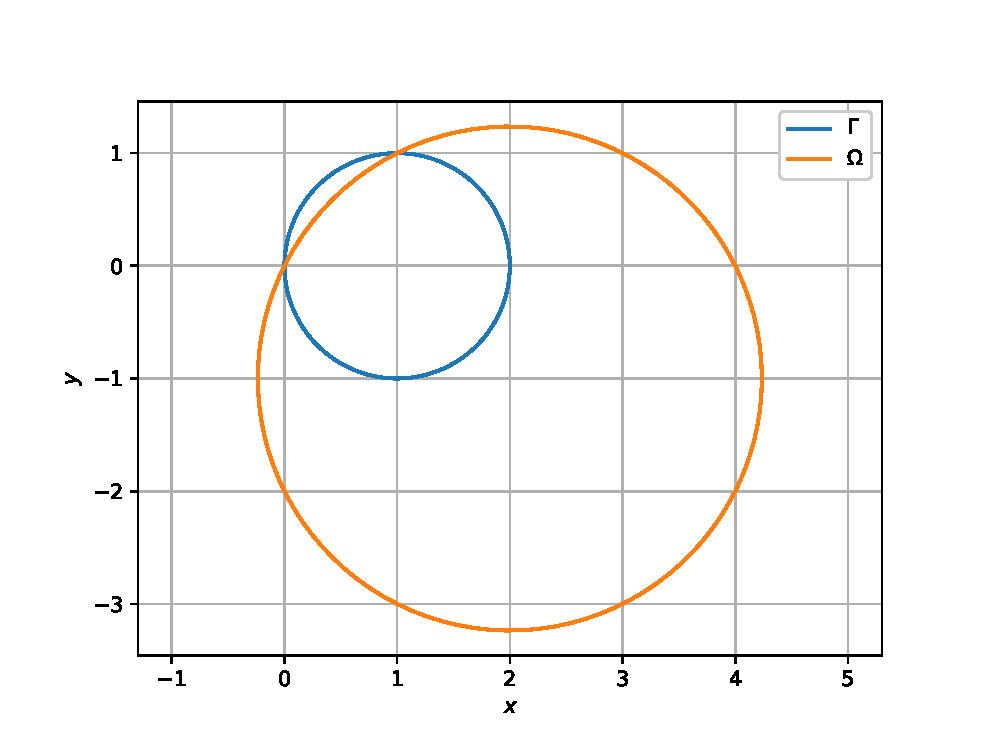
\includegraphics[width=\columnwidth]{./figs/2019_1_1.eps}
\caption{}
\label{fig:2019_1}
\end{figure}
%
\item Obtain the Lagrangian.
\\
\solution
The Lagrangian is 
\begin{align}
L \brak{\vec{x},\lambda} = \norm{\vec{x} - \vec{c}_1}^2 - \lambda 
\cbrak{\norm{\vec{x} - \vec{c}_2}^2-r_2^2}
\end{align}
\item Use the KKT conditions to obtain the minima.
\\
\solution
From the KKT conditions, 
\begin{align}
\frac{\partial L \brak{\vec{x},\lambda}}{\partial \vec{x}} &= 0
\\
\implies {\vec{x} - \vec{c}_1} - \lambda \brak{\vec{x} - \vec{c}_2} &= 0
\\
\implies \vec{x}  = \frac{\vec{c}_1 -\lambda  \vec{c}_2}{1-\lambda } &
\label{eq:opt_xlam}
\end{align}
%
and 
\begin{align}
\frac{\partial L \brak{\vec{x},\lambda}}{\partial \lambda} &= 0
\\
\implies \norm{\vec{x} - \vec{c}_2}^2-r_2^2 &= 0
\label{eq:opt_xnorm}
\end{align}
Substituting from \eqref{eq:opt_xlam} in \eqref{eq:opt_xnorm},
\begin{align}
\norm{\frac{\vec{c}_1 -\lambda  \vec{c}_2}{1-\lambda } - \vec{c}_2}^2-r_2^2 &= 0
\\
\implies \lambda = 1\pm \frac{\norm{\vec{c}_1 - \vec{c}_2}}{r_2}&
\\
= 1 \pm \sqrt{\frac{2}{5}}
%\label{eq:opt_xnorm}
\end{align}
Fig. \ref{fig:2019_1_2} plots $\Gamma$ for 
\begin{align}
\lambda = 1 - \sqrt{\frac{2}{5}}
\end{align}
\item If the maximum value is obtained at $z_0$, find the principal argument of
\begin{align}
\frac{4 - z_0-\bar{z}_0}{z_0-\bar{z}_0+2\j}
\end{align}
\\
\solution 
From \eqref{eq:opt_xlam},
\begin{align}
 \vec{x}_0  &= \frac{\vec{c}_1 -\lambda  \vec{c}_2}{1-\lambda } 
\\
\implies z_0 &= \frac{1}{1-\lambda}\brak{1-2\lambda + \j \lambda }
\\
\text{or, }\arg \frac{4 - z_0-\bar{z}_0}{z_0-\bar{z}_0+2\j} &= \frac{2 - \Re\cbrak{z_0}}{\j\brak{\Im\cbrak{z_0}+1}}
\\
&=\frac{2\brak{1-\lambda}-\brak{1-2\lambda}}{\j} 
\\
&= -\j
\end{align}
%
Thus, the principal argument is $-\frac{\pi}{2}$.
\begin{figure}[!ht]
\centering
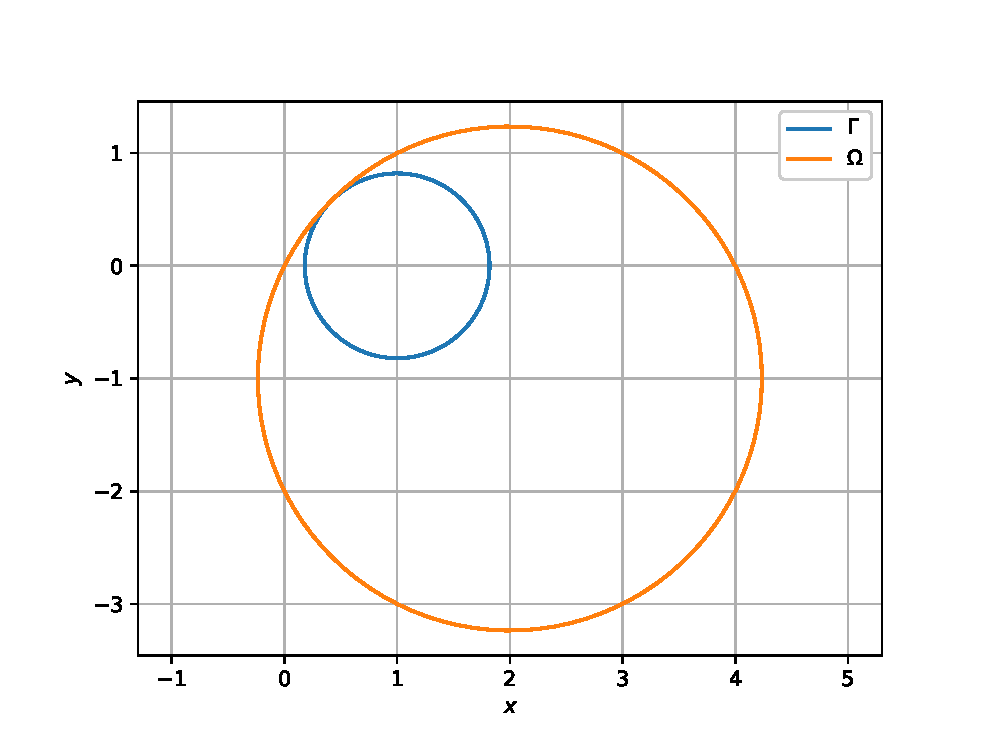
\includegraphics[width=\columnwidth]{./figs/2019_1_2.eps}
\caption{}
\label{fig:2019_1_2}
\end{figure}

%\begin{enumerate}[label=\theenumi.\arabic*
%,ref=\thesection.\theenumi]
\item Show that the set 
\begin{align}
D = \cbrak{\vec{x}:\norm{\vec{x}-\vec{C}_2} \ge r_2}, r_2 > 0
\end{align}
%
is nonconvex.
\\
\solution Let $\vec{x}_1 \in D$ and 
\begin{align}
\vec{x}_2 = 2\vec{C}_2-\vec{x}_1
\end{align}
Then 
\begin{align}
\norm{\vec{x}_2-\vec{C}_2} &= \norm{\vec{C}_2-\vec{x}_1} \ge r_2
\\
\implies \vec{x}_2 &\in D.
\end{align}
Suppose 
\begin{align}
\vec{x} = \theta\vec{x}_1+\brak{1-\theta}\vec{x}_2
\end{align}
For $\theta = \frac{1}{2}$,
\begin{align}
\vec{x} &= \vec{C}_2
\\
\implies \norm{\vec{x}-\vec{C}_2} &= 0,
\\
\text{or, } \vec{x} &\notin D
\end{align}
Thus, by definition, $D$ is not a convex set.
\end{enumerate}
%and is sketched in Fig. \ref{fig:2019_opt_fun}.
\section{Matrices: Cayley-Hamilton Theorem}
\begin{enumerate}[label=\thesection.\arabic*
,ref=\thesection.\theenumi]

\item Let
\begin{align}
\label{eq:mat_def}
\vec{M} = \myvec{\sin^4\theta & -1-\sin^2\theta \\ 1+ \cos^2\theta & \cos^4\theta} = \alpha\vec{I} + \beta \vec{M}^{-1}
\end{align}
where $\alpha, \beta$ are real functions of $\theta$ and $\vec{I}$ is the identity matrix. Find the characteristic equation of $\vec{M}$.
\\
\solution \eqref{eq:mat_def} can be expressed as
\begin{align}
\vec{M}^2 -\alpha\vec{M} - \beta \vec{I} = 0
\end{align}
%
which yields   the characteristic equation of $\vec{M}$ as
\begin{align}
\lambda^2 -\alpha\lambda - \beta  = 0
\end{align}
\item Find $\alpha$ and $\beta$.
\\
\solution
Since the sum of the eigenvalues is equal to the trace and the determinant is the product of eigenvalues,
\begin{align}
 \alpha &= \sin^4\theta + \cos^4\theta 
\\
  \beta & = -\sin^4\theta \cos^4\theta + \brak{1+\sin^2\theta}\brak{ 1+ \cos^2\theta}
\end{align}
\item If 
\begin{align}
\alpha^{*} &= \min_{\theta}\alpha\brak{\theta}
\\
\beta^{*} &= \min_{\theta}\beta\brak{\theta}, 
\end{align}
find $\alpha^{*} + \beta^{*}$.
\\
\solution 
\begin{align}
\because  \alpha &= \sin^4\theta + \cos^4\theta = 1 - \frac{\sin^2 2\theta}{2},
\\
\alpha^{*} &= \frac{1}{2}, 
\end{align}
Similarly,
\begin{align}
 - \beta & = \sin^4\theta \cos^4\theta + \brak{1+\sin^2\theta}\brak{ 1+ \cos^2\theta}
\\
&=2 + \frac{\sin^2 2\theta}{4} + \frac{\sin^4 2\theta}{16}
\\
&= \brak{\frac{\sin^2 2\theta}{4}+\frac{1}{2}}^2+ \frac{7}{4} 
\end{align}
Thus,
\begin{align}
 \beta^{*} &= -\frac{37}{16}
\\
\implies \alpha^{*}+\beta^{*} &= -\frac{29}{16}
\end{align}
\end{enumerate}
\section{Vector Algebra}
\begin{enumerate}[label=\thesection.\arabic*
,ref=\thesection.\theenumi]

\item The line 
\begin{align}
\Gamma: \vec{x} = \myvec{0 \\ 1} + \lambda \myvec{1 \\ m}
\label{eq:coord_line}
\end{align}
intersects the circle
\begin{align}
\Omega: \norm{\vec{x}-\myvec{3 \\ -2}} = 5
\label{eq:coord_circ}
\end{align}
at points $\vec{P}$ and $\vec{Q}$ respectively. The mid point of $PQ$ is 
$\vec{R}$ such that
\begin{align}
\myvec{1 & 0}\vec{R} = -\frac{3}{5}
\label{eq:coord_mid}
\end{align}
%
Find $m$.
\\
\solution Let 
\begin{align}
\vec{c} = \myvec{0 \\ 1}, \vec{O} = \myvec{3 \\ -2} \text{ and } \vec{m} = 
\myvec{1 \\ m}
\label{eq:coord_defs}
\end{align}
%
The intersection of  \eqref{eq:coord_line} and \eqref{eq:coord_circ} is 
\begin{align}
\norm{\vec{c}+\lambda\vec{m} -\vec{O}}^2 = 25
\end{align}
\begin{multline}
\label{eq:coord_quad}
\implies \lambda^2 \norm{\vec{m}}^2+ 2\lambda\vec{m}^{T}\brak{\vec{c} 
-\vec{O}}
\\
+\norm{\vec{c} -\vec{O}}^2-25 = 0
\end{multline}
%
Since $\vec{P}, \vec{Q}$ lie on $\Gamma$,
\begin{align}
\vec{P} &= \vec{c}+\lambda_1\vec{m} 
\\
\vec{Q} &= \vec{c}+\lambda_2\vec{m} 
\\
\implies \frac{\vec{P}+\vec{Q}}{2} &= \vec{c} + 
\frac{\lambda_1+\lambda_2}{2}\vec{m} 
\\
\implies \myvec{1 & 0}\frac{\vec{P}+\vec{Q}}{2} &= \myvec{1 & 0}\vec{c}
\nonumber \\
& \,+ \frac{\lambda_1+\lambda_2}{2}\myvec{1 & 0}\vec{m} 
\\
&= \myvec{1 & 0}\vec{c} -
\frac{\vec{m}^{T}\brak{\vec{c} -\vec{O}}}{\norm{\vec{m}}^2}
\end{align}
using the sum of roots in \eqref{eq:coord_quad}.  From 
\eqref{eq:coord_mid} and \eqref{eq:coord_defs},
\begin{align}
-\myvec{1 & m}\myvec{-3\\3}= -\frac{3}{5}\brak{1+m^2}
\\
\implies m^2 -5m + 6 = 0
\\
\implies m = 2 \text{ or } 3
\end{align}
From \eqref{eq:coord_quad}, 
\begin{multline}
\lambda = \frac{-\vec{m}^{T}\brak{\vec{c} -\vec{O}}}{{\norm{\vec{m}}^2}}
\\
\pm \frac{\sqrt{\brak{\vec{m}^{T}\brak{\vec{c} -\vec{O}}}^2
-\norm{\vec{c} -\vec{O}}^2+25}}{\norm{\vec{m}}^2}
\end{multline}
Fig. \ref{fig:2019_3} summarizes the solution for $m = 2$.

%\renewcommand\thefigure{\theenumi}

\begin{figure}
\centering
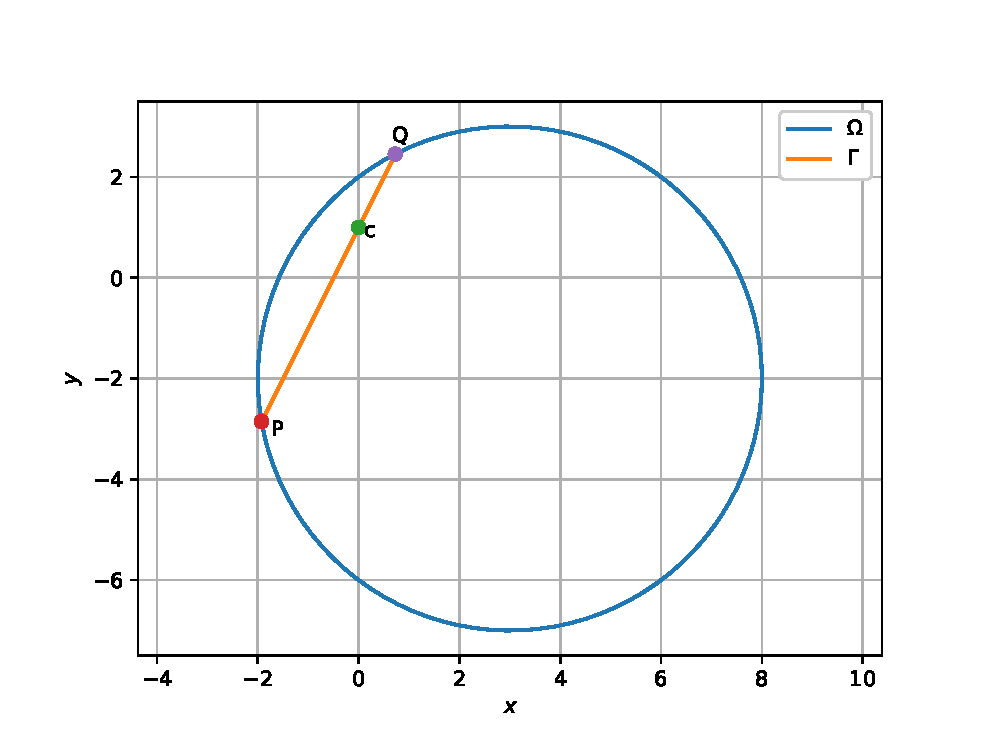
\includegraphics[width=\columnwidth]{./figs/2019_3.eps}
\caption{}
\label{fig:2019_3}
\end{figure}
\end{enumerate}
\section{Calculus: Integration}
\begin{enumerate}[label=\thesection.\arabic*
,ref=\thesection.\theenumi]

\item Sketch the region 
\begin{align}
\myvec{x \\ y}: xy \le 8, 1\le y \le x^2
\end{align}
%
\item Find the area of the region.
\\ 
\solution The intersection of $y = 1, y = x^2$ is
\begin{align}
\vec{A} = \myvec{1 \\ 1}
\end{align}
The intersection of $y = 1, xy = 8$ is
\begin{align}
\vec{B} = \myvec{8 \\ 1}
\end{align}
%%
The intersection of $y = x^2, xy = 8$ is
\begin{align}
\vec{C} = \myvec{2 \\ 4}
\end{align}
%
The desired region is enclosed by the vertices $\vec{A},\vec{B}$ and 
$\vec{C}$
\begin{figure}
\centering
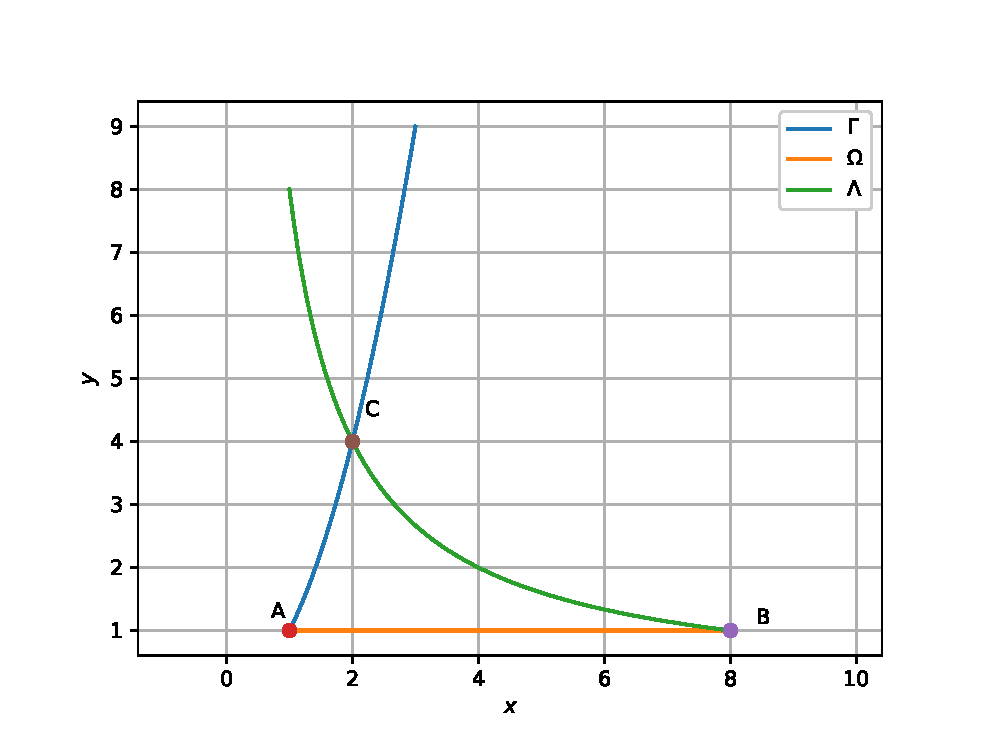
\includegraphics[width=\columnwidth]{./figs/2019_4.eps}
\caption{}
\label{fig:2019_4}
\end{figure}
%
Thus, the area is obtained as
\begin{align}
\int_{1}^{2}x^2\,dx + \int_{2}^{8}\frac{8}{x}\,dx
&= \sbrak{\frac{x^3}{3}}_{1}^{2}+8 \sbrak{\ln x}_{2}^{8} - 7
\\
&= 16 \ln 2 - \frac{14}{3}
\end{align}
\end{enumerate}
\section{Signal Processing: Z Transform}
\begin{enumerate}[label=\thesection.\arabic*
,ref=\thesection.\theenumi]

\item Let
\begin{align}
a(n) &= \frac{\alpha^n-\beta^n}{\alpha-\beta}u(n)
\\
b(n) &=a(n-1)+a(n+1) - \delta(n)
\end{align}
where $\alpha, \beta$ are the roots of the equation
\begin{equation}
z^2-z-1 = 0
\end{equation}
and
\begin{align}
u(n)
=
\begin{cases}
0, & n < 0
\\
1, & n \ge 0
\end{cases}
\\
\delta(n)
=
\begin{cases}
0, & n \ne 0
\\
1, & n = 0
\end{cases}
\end{align}
\item Verify your results through a C program.
%\begin{enumerate}[label=\theenumi.\arabic*
%,ref=\thesection.\theenumi]
\item Show that the $Z$ transform of $u(n)$
\begin{align}
U(z)&\triangleq \sum_{n=-\infty}^{\infty}u(n)z^{-n} 
\\
&= \frac{1}{1- z^{-1}}, \quad \abs{z} > 1
\end{align}
\item  Show that 
\begin{align}
A(z)&= \frac{z^{-1}}{1- z^{-1}-z^{-2}}
\end{align}
\item Let 
\begin{align}
y(n)=a(n)*u(n) \triangleq \sum_{k=-\infty}^{\infty}a(k) u(n-k)
\end{align}
%
Show that 
\begin{align}
y(n) = \sum_{k=0}^{n}a(k) 
\end{align}
%
\item Show that 
\begin{align}
Y(z) &= A(z)U(z)
\\
&= \frac{z^{-1}}{\brak{1- z^{-1}-z^{-2}}\brak{1- z^{-1}}}
\end{align}
\item Show that 
\begin{align}
w(n)&=\sbrak{a(n+2)-1}u(n-1)
\\
&=a(n+2)-u(n+1)+2\delta(n)
\end{align}
\item Is $W(z)=Y(z)$?
\item Verify if 
\begin{align}
\sum_{n=1}^{\infty}\frac{a(n)}{10^n} = \frac{10}{89}
\end{align}
\item Verify if 
\begin{align}
\sum_{n=1}^{\infty}\frac{b(n)}{10^n} = \frac{8}{89}
\end{align}

\end{enumerate}
\section{Matrices: Adjugate}
Let 
\begin{align}
\vec{M} = \myvec{0 & 1 & a \\ 1 & 2 & 3 \\ 3 & b & 1}, \quad 
\text{ adj}\brak{\vec{M}} = \myvec{-1 & 1 & -1 \\ 8 & -6 & 2 \\ -5 & 3 & -1}
\end{align}
\begin{enumerate}[label=\thesection.\arabic*
,ref=\thesection.\theenumi]
\item Show that $a+b = 3$
\\
\solution 
\begin{align}
\label{eq:adj_Minv}
\because \vec{M} \text{ adj}\brak{\vec{M}} &= \det \brak{\vec{M}}\vec{I},
%\\
%\myvec{0 & 1 & a }
% \myvec{-1 \\ 8 \\ -5 } &= \det \brak{\vec{M}}
\\
\myvec{0 & 1 & a } 
 \myvec{1 \\ -6 \\ 3} &= 0
\\
\myvec{3 & b & 1 } 
 \myvec{-1 \\ 8 \\ -5} &= 0
\end{align}
%
resulting in 
\begin{align}
a = 2, b = 1
\end{align}
Hence, $a+b = 3$.
\item Verify if 
\begin{align}
\brak{\text{ adj}\brak{\vec{M}}}^{-1} + \text{ adj}\brak{\vec{M}^{-1}} = -\vec{M}
\end{align}
\\
\solution From \eqref{eq:adj_Minv}
\begin{align}
\brak{\text{ adj}\brak{\vec{M}}}^{-1} = \frac{\vec{M}}{\det\brak{\vec{M}}}
\end{align}
%
and 
\begin{align}
\brak{\text{ adj}\brak{\vec{M}^{-1}}} &= \frac{\vec{M}^{-1}}{\det\brak{\vec{M}^{-1}}}
\\
&= {\vec{M}^{-1}}{\det\brak{\vec{M}}}
\end{align}
%
Thus, 
\begin{multline}
\brak{\text{ adj}\brak{\vec{M}^{-1}}} + \text{ adj}\brak{\vec{M}^{-1}}
\\
= {\vec{M}^{-1}}{\det\brak{\vec{M}}}+\frac{\vec{M}}{\det\brak{\vec{M}}}
\\
= \text{ adj}\brak{\vec{M}}+\frac{\vec{M}}{\det\brak{\vec{M}}}
\end{multline}
From \eqref{eq:adj_Minv}
\begin{align}
\myvec{0 & 1 & a } 
 \myvec{-1 \\ 8 \\ -5} &= \det\brak{\vec{M}}
\\
\implies \det\brak{\vec{M}} = 8-5a &= -2
\end{align}
If
\begin{align*}
\brak{\text{ adj}\brak{\vec{M}^{-1}}} + \text{ adj}\brak{\vec{M}^{-1}}
&= -\vec{M},
\\
\text{ adj}\brak{\vec{M}}-\frac{\vec{M}}{2} &=  -\vec{M}
\\
\implies \vec{M} &= - \text{ adj}\brak{\vec{M}}
\end{align*}
%
which is incorrect.
\item Verify if
\begin{align}
\det\brak{\text{ adj}\brak{\vec{M}^2}}  = 81
\end{align}
\solution 
\begin{align}
\text{ adj}\brak{\vec{M}^2}  &= \vec{M}^{-2}\det\brak{\vec{M}}^{2}
\\
&= 4{\vec{M}^{-2}}
\\
\implies \det\brak{\text{ adj}\brak{\vec{M}^2}}  &= 4^3\det\brak{\vec{M}}^{-2}
\\
&= 16 \ne 81
\end{align}
%
\item If 
\begin{align}
\vec{M}\myvec{\alpha \\ \beta \\ \gamma}  = \myvec{1 \\ 2 \\ 3}, 
\end{align}
show that 
\begin{align}
\alpha - \beta + \gamma = 3
\end{align}
\solution 
\begin{align}
\vec{M}\myvec{\alpha \\ \beta \\ \gamma}  &= \myvec{1 \\ 2 \\ 3}, 
\\
\implies \text{ adj}\brak{\vec{M}}\vec{M}\myvec{\alpha \\ \beta \\ \gamma}  &= \text{ adj}\brak{\vec{M}}\myvec{1 \\ 2 \\ 3}, 
\end{align}
%
which can be expressed as
\begin{align}
 \det\brak{\vec{M}}\myvec{\alpha \\ \beta \\ \gamma}  &= \text{ adj}\brak{\vec{M}}\myvec{1 \\ 2 \\ 3}, 
\\
\text{or, } \myvec{\alpha \\ \beta \\ \gamma} &= -\frac{1}{2}\text{ adj}\brak{\vec{M}}\myvec{1 \\ 2 \\ 3}, 
\end{align}
Thus, 
\begin{align}
\alpha - \beta + \gamma &= \myvec{1 & -1& 1} \myvec{\alpha \\ \beta \\ \gamma} 
\\
&=-\frac{1}{2}\myvec{1 & -1& 1}\text{ adj}\brak{\vec{M}}\myvec{1 \\ 2 \\ 3}
\\
&=\myvec{7 & -5& 2}\myvec{1 \\ 2 \\ 3}
=3
\end{align}
\end{enumerate}
\section{Probability}
Table \ref{table:2019_7} lists the number of red (R) and green (G) balls in bags $B_1, B_2$ and $B_3$. Also listed are the probabilities of each bag.
\begin{table}[!h]
\centering
%\resizebox {0.5\columnwidth} {!} {
%%%%%%%%%%%%%%%%%%%%%%%%%%%%%%%%%%%%%%%%%%%%%%%%%%%%%%%%%%%%%%%%%%%%%%%
%%                                                                  %%
%%  This is the header of a LaTeX2e file exported from Gnumeric.    %%
%%                                                                  %%
%%  This file can be compiled as it stands or included in another   %%
%%  LaTeX document. The table is based on the longtable package so  %%
%%  the longtable options (headers, footers...) can be set in the   %%
%%  preamble section below (see PRAMBLE).                           %%
%%                                                                  %%
%%  To include the file in another, the following two lines must be %%
%%  in the including file:                                          %%
%%        \def\inputGnumericTable{}                                 %%
%%  at the beginning of the file and:                               %%
%%        \input{name-of-this-file.tex}                             %%
%%  where the table is to be placed. Note also that the including   %%
%%  file must use the following packages for the table to be        %%
%%  rendered correctly:                                             %%
%%    \usepackage[latin1]{inputenc}                                 %%
%%    \usepackage{color}                                            %%
%%    \usepackage{array}                                            %%
%%    \usepackage{longtable}                                        %%
%%    \usepackage{calc}                                             %%
%%    \usepackage{multirow}                                         %%
%%    \usepackage{hhline}                                           %%
%%    \usepackage{ifthen}                                           %%
%%  optionally (for landscape tables embedded in another document): %%
%%    \usepackage{lscape}                                           %%
%%                                                                  %%
%%%%%%%%%%%%%%%%%%%%%%%%%%%%%%%%%%%%%%%%%%%%%%%%%%%%%%%%%%%%%%%%%%%%%%



%%  This section checks if we are begin input into another file or  %%
%%  the file will be compiled alone. First use a macro taken from   %%
%%  the TeXbook ex 7.7 (suggestion of Han-Wen Nienhuys).            %%
\def\ifundefined#1{\expandafter\ifx\csname#1\endcsname\relax}


%%  Check for the \def token for inputed files. If it is not        %%
%%  defined, the file will be processed as a standalone and the     %%
%%  preamble will be used.                                          %%
\ifundefined{inputGnumericTable}

%%  We must be able to close or not the document at the end.        %%
	\def\gnumericTableEnd{\end{document}}


%%%%%%%%%%%%%%%%%%%%%%%%%%%%%%%%%%%%%%%%%%%%%%%%%%%%%%%%%%%%%%%%%%%%%%
%%                                                                  %%
%%  This is the PREAMBLE. Change these values to get the right      %%
%%  paper size and other niceties.                                  %%
%%                                                                  %%
%%%%%%%%%%%%%%%%%%%%%%%%%%%%%%%%%%%%%%%%%%%%%%%%%%%%%%%%%%%%%%%%%%%%%%

	\documentclass[12pt%
			  %,landscape%
                    ]{report}
       \usepackage[latin1]{inputenc}
       \usepackage{fullpage}
       \usepackage{color}
       \usepackage{array}
       \usepackage{longtable}
       \usepackage{calc}
       \usepackage{multirow}
       \usepackage{hhline}
       \usepackage{ifthen}

	\begin{document}


%%  End of the preamble for the standalone. The next section is for %%
%%  documents which are included into other LaTeX2e files.          %%
\else

%%  We are not a stand alone document. For a regular table, we will %%
%%  have no preamble and only define the closing to mean nothing.   %%
    \def\gnumericTableEnd{}

%%  If we want landscape mode in an embedded document, comment out  %%
%%  the line above and uncomment the two below. The table will      %%
%%  begin on a new page and run in landscape mode.                  %%
%       \def\gnumericTableEnd{\end{landscape}}
%       \begin{landscape}


%%  End of the else clause for this file being \input.              %%
\fi

%%%%%%%%%%%%%%%%%%%%%%%%%%%%%%%%%%%%%%%%%%%%%%%%%%%%%%%%%%%%%%%%%%%%%%
%%                                                                  %%
%%  The rest is the gnumeric table, except for the closing          %%
%%  statement. Changes below will alter the table's appearance.     %%
%%                                                                  %%
%%%%%%%%%%%%%%%%%%%%%%%%%%%%%%%%%%%%%%%%%%%%%%%%%%%%%%%%%%%%%%%%%%%%%%

\providecommand{\gnumericmathit}[1]{#1} 
%%  Uncomment the next line if you would like your numbers to be in %%
%%  italics if they are italizised in the gnumeric table.           %%
%\renewcommand{\gnumericmathit}[1]{\mathit{#1}}
\providecommand{\gnumericPB}[1]%
{\let\gnumericTemp=\\#1\let\\=\gnumericTemp\hspace{0pt}}
 \ifundefined{gnumericTableWidthDefined}
        \newlength{\gnumericTableWidth}
        \newlength{\gnumericTableWidthComplete}
        \newlength{\gnumericMultiRowLength}
        \global\def\gnumericTableWidthDefined{}
 \fi
%% The following setting protects this code from babel shorthands.  %%
 \ifthenelse{\isundefined{\languageshorthands}}{}{\languageshorthands{english}}
%%  The default table format retains the relative column widths of  %%
%%  gnumeric. They can easily be changed to c, r or l. In that case %%
%%  you may want to comment out the next line and uncomment the one %%
%%  thereafter                                                      %%
\providecommand\gnumbox{\makebox[0pt]}
%%\providecommand\gnumbox[1][]{\makebox}

%% to adjust positions in multirow situations                       %%
\setlength{\bigstrutjot}{\jot}
\setlength{\extrarowheight}{\doublerulesep}

%%  The \setlongtables command keeps column widths the same across  %%
%%  pages. Simply comment out next line for varying column widths.  %%
\setlongtables

\setlength\gnumericTableWidth{%
	140pt+%
	44pt+%
0pt}
\def\gumericNumCols{2}
\setlength\gnumericTableWidthComplete{\gnumericTableWidth+%
         \tabcolsep*\gumericNumCols*2+\arrayrulewidth*\gumericNumCols}
\ifthenelse{\lengthtest{\gnumericTableWidthComplete > \linewidth}}%
         {\def\gnumericScale{\ratio{\linewidth-%
                        \tabcolsep*\gumericNumCols*2-%
                        \arrayrulewidth*\gumericNumCols}%
{\gnumericTableWidth}}}%
{\def\gnumericScale{1}}

%%%%%%%%%%%%%%%%%%%%%%%%%%%%%%%%%%%%%%%%%%%%%%%%%%%%%%%%%%%%%%%%%%%%%%
%%                                                                  %%
%% The following are the widths of the various columns. We are      %%
%% defining them here because then they are easier to change.       %%
%% Depending on the cell formats we may use them more than once.    %%
%%                                                                  %%
%%%%%%%%%%%%%%%%%%%%%%%%%%%%%%%%%%%%%%%%%%%%%%%%%%%%%%%%%%%%%%%%%%%%%%

\ifthenelse{\isundefined{\gnumericColA}}{\newlength{\gnumericColA}}{}\settowidth{\gnumericColA}{\begin{tabular}{@{}p{140pt*\gnumericScale}@{}}x\end{tabular}}
\ifthenelse{\isundefined{\gnumericColB}}{\newlength{\gnumericColB}}{}\settowidth{\gnumericColB}{\begin{tabular}{@{}p{44pt*\gnumericScale}@{}}x\end{tabular}}


\begin{tabular}[c]{%
%begin{longtable}[c]{%
	b{\gnumericColA}%
	b{\gnumericColB}%
	}

%%%%%%%%%%%%%%%%%%%%%%%%%%%%%%%%%%%%%%%%%%%%%%%%%%%%%%%%%%%%%%%%%%%%%%
%%  The longtable options. (Caption, headers... see Goosens, p.124) %%
%	\caption{The Table Caption.}             \\	%
% \hline	% Across the top of the table.
%%  The rest of these options are table rows which are placed on    %%
%%  the first, last or every page. Use \multicolumn if you want.    %%

%%  Header for the first page.                                      %%
%	\multicolumn{2}{c}{The First Header} \\ \hline 
%	\multicolumn{1}{c}{colTag}	%Column 1
%	&\multicolumn{1}{c}{colTag}	\\ \hline %Last column
%	\endfirsthead

%%  The running header definition.                                  %%
%	\hline
%	\multicolumn{2}{l}{\ldots\small\slshape continued} \\ \hline
%	\multicolumn{1}{c}{colTag}	%Column 1
%	&\multicolumn{1}{c}{colTag}	\\ \hline %Last column
%	\endhead

%%  The running footer definition.                                  %%
%	\hline
%	\multicolumn{2}{r}{\small\slshape continued\ldots} \\
%	\endfoot

%%  The ending footer definition.                                   %%
%	\multicolumn{2}{c}{That's all folks} \\ \hline 
%	\endlastfoot
%%%%%%%%%%%%%%%%%%%%%%%%%%%%%%%%%%%%%%%%%%%%%%%%%%%%%%%%%%%%%%%%%%%%%%

\hhline{|-|-}
	 \multicolumn{1}{|p{\gnumericColA}|}%
	{\gnumericPB{\raggedright}\gnumbox[l]{\textbf{Component}}}
	&\multicolumn{1}{p{\gnumericColB}|}%
	{\gnumericPB{\raggedright}\gnumbox[l]{\textbf{Quantity}}}
\\
\hhline{|--|}
	 \multicolumn{1}{|p{\gnumericColA}|}%
	{\gnumericPB{\raggedright}\gnumbox[l]{STM32F103C8T6}}
	&\multicolumn{1}{p{\gnumericColB}|}%
	{\gnumericPB{\raggedleft}\gnumbox[r]{1}}
\\
\hhline{|--|}
	 \multicolumn{1}{|p{\gnumericColA}|}%
	{\gnumericPB{\raggedright}\gnumbox[l]{Raspberry Pi 3}}
	&\multicolumn{1}{p{\gnumericColB}|}%
	{\gnumericPB{\raggedleft}\gnumbox[r]{1}}
\\
\hhline{|--|}
	 \multicolumn{1}{|p{\gnumericColA}|}%
	{\gnumericPB{\raggedright}\gnumbox[l]{STLINK V2}}
	&\multicolumn{1}{p{\gnumericColB}|}%
	{\gnumericPB{\raggedleft}\gnumbox[r]{1}}
\\
\hhline{|--|}
	 \multicolumn{1}{|p{\gnumericColA}|}%
	{\gnumericPB{\raggedright}\gnumbox[l]{Female-Female Jumper Wires}}
	&\multicolumn{1}{p{\gnumericColB}|}%
	{\gnumericPB{\raggedleft}\gnumbox[r]{5}}
\\
\hhline{|-|-|}
\end{tabular}
%\end{longtable}

\ifthenelse{\isundefined{\languageshorthands}}{}{\languageshorthands{\languagename}}
\gnumericTableEnd

%%%%%%%%%%%%%%%%%%%%%%%%%%%%%%%%%%%%%%%%%%%%%%%%%%%%%%%%%%%%%%%%%%%%%%
%%                                                                  %%
%%  This is the header of a LaTeX2e file exported from Gnumeric.    %%
%%                                                                  %%
%%  This file can be compiled as it stands or included in another   %%
%%  LaTeX document. The table is based on the longtable package so  %%
%%  the longtable options (headers, footers...) can be set in the   %%
%%  preamble section below (see PRAMBLE).                           %%
%%                                                                  %%
%%  To include the file in another, the following two lines must be %%
%%  in the including file:                                          %%
%%        \def\inputGnumericTable{}                                 %%
%%  at the beginning of the file and:                               %%
%%        \input{name-of-this-file.tex}                             %%
%%  where the table is to be placed. Note also that the including   %%
%%  file must use the following packages for the table to be        %%
%%  rendered correctly:                                             %%
%%    \usepackage[latin1]{inputenc}                                 %%
%%    \usepackage{color}                                            %%
%%    \usepackage{array}                                            %%
%%    \usepackage{longtable}                                        %%
%%    \usepackage{calc}                                             %%
%%    \usepackage{multirow}                                         %%
%%    \usepackage{hhline}                                           %%
%%    \usepackage{ifthen}                                           %%
%%  optionally (for landscape tables embedded in another document): %%
%%    \usepackage{lscape}                                           %%
%%                                                                  %%
%%%%%%%%%%%%%%%%%%%%%%%%%%%%%%%%%%%%%%%%%%%%%%%%%%%%%%%%%%%%%%%%%%%%%%



%%  This section checks if we are begin input into another file or  %%
%%  the file will be compiled alone. First use a macro taken from   %%
%%  the TeXbook ex 7.7 (suggestion of Han-Wen Nienhuys).            %%
\def\ifundefined#1{\expandafter\ifx\csname#1\endcsname\relax}


%%  Check for the \def token for inputed files. If it is not        %%
%%  defined, the file will be processed as a standalone and the     %%
%%  preamble will be used.                                          %%
\ifundefined{inputGnumericTable}

%%  We must be able to close or not the document at the end.        %%
	\def\gnumericTableEnd{\end{document}}


%%%%%%%%%%%%%%%%%%%%%%%%%%%%%%%%%%%%%%%%%%%%%%%%%%%%%%%%%%%%%%%%%%%%%%
%%                                                                  %%
%%  This is the PREAMBLE. Change these values to get the right      %%
%%  paper size and other niceties.                                  %%
%%                                                                  %%
%%%%%%%%%%%%%%%%%%%%%%%%%%%%%%%%%%%%%%%%%%%%%%%%%%%%%%%%%%%%%%%%%%%%%%

	\documentclass[12pt%
			  %,landscape%
                    ]{report}
       \usepackage[latin1]{inputenc}
       \usepackage{fullpage}
       \usepackage{color}
       \usepackage{array}
       \usepackage{longtable}
       \usepackage{calc}
       \usepackage{multirow}
       \usepackage{hhline}
       \usepackage{ifthen}

	\begin{document}


%%  End of the preamble for the standalone. The next section is for %%
%%  documents which are included into other LaTeX2e files.          %%
\else

%%  We are not a stand alone document. For a regular table, we will %%
%%  have no preamble and only define the closing to mean nothing.   %%
    \def\gnumericTableEnd{}

%%  If we want landscape mode in an embedded document, comment out  %%
%%  the line above and uncomment the two below. The table will      %%
%%  begin on a new page and run in landscape mode.                  %%
%       \def\gnumericTableEnd{\end{landscape}}
%       \begin{landscape}


%%  End of the else clause for this file being \input.              %%
\fi

%%%%%%%%%%%%%%%%%%%%%%%%%%%%%%%%%%%%%%%%%%%%%%%%%%%%%%%%%%%%%%%%%%%%%%
%%                                                                  %%
%%  The rest is the gnumeric table, except for the closing          %%
%%  statement. Changes below will alter the table's appearance.     %%
%%                                                                  %%
%%%%%%%%%%%%%%%%%%%%%%%%%%%%%%%%%%%%%%%%%%%%%%%%%%%%%%%%%%%%%%%%%%%%%%

\providecommand{\gnumericmathit}[1]{#1} 
%%  Uncomment the next line if you would like your numbers to be in %%
%%  italics if they are italizised in the gnumeric table.           %%
%\renewcommand{\gnumericmathit}[1]{\mathit{#1}}
\providecommand{\gnumericPB}[1]%
{\let\gnumericTemp=\\#1\let\\=\gnumericTemp\hspace{0pt}}
 \ifundefined{gnumericTableWidthDefined}
        \newlength{\gnumericTableWidth}
        \newlength{\gnumericTableWidthComplete}
        \newlength{\gnumericMultiRowLength}
        \global\def\gnumericTableWidthDefined{}
 \fi
%% The following setting protects this code from babel shorthands.  %%
 \ifthenelse{\isundefined{\languageshorthands}}{}{\languageshorthands{english}}
%%  The default table format retains the relative column widths of  %%
%%  gnumeric. They can easily be changed to c, r or l. In that case %%
%%  you may want to comment out the next line and uncomment the one %%
%%  thereafter                                                      %%
\providecommand\gnumbox{\makebox[0pt]}
%%\providecommand\gnumbox[1][]{\makebox}

%% to adjust positions in multirow situations                       %%
\setlength{\bigstrutjot}{\jot}
\setlength{\extrarowheight}{\doublerulesep}

%%  The \setlongtables command keeps column widths the same across  %%
%%  pages. Simply comment out next line for varying column widths.  %%
\setlongtables

\setlength\gnumericTableWidth{%
	28pt+%
	12pt+%
	13pt+%
	75pt+%
0pt}
\def\gumericNumCols{4}
\setlength\gnumericTableWidthComplete{\gnumericTableWidth+%
         \tabcolsep*\gumericNumCols*2+\arrayrulewidth*\gumericNumCols}
\ifthenelse{\lengthtest{\gnumericTableWidthComplete > \linewidth}}%
         {\def\gnumericScale{\ratio{\linewidth-%
                        \tabcolsep*\gumericNumCols*2-%
                        \arrayrulewidth*\gumericNumCols}%
{\gnumericTableWidth}}}%
{\def\gnumericScale{1}}

%%%%%%%%%%%%%%%%%%%%%%%%%%%%%%%%%%%%%%%%%%%%%%%%%%%%%%%%%%%%%%%%%%%%%%
%%                                                                  %%
%% The following are the widths of the various columns. We are      %%
%% defining them here because then they are easier to change.       %%
%% Depending on the cell formats we may use them more than once.    %%
%%                                                                  %%
%%%%%%%%%%%%%%%%%%%%%%%%%%%%%%%%%%%%%%%%%%%%%%%%%%%%%%%%%%%%%%%%%%%%%%

\ifthenelse{\isundefined{\gnumericColA}}{\newlength{\gnumericColA}}{}\settowidth{\gnumericColA}{\begin{tabular}{@{}p{28pt*\gnumericScale}@{}}x\end{tabular}}
\ifthenelse{\isundefined{\gnumericColB}}{\newlength{\gnumericColB}}{}\settowidth{\gnumericColB}{\begin{tabular}{@{}p{12pt*\gnumericScale}@{}}x\end{tabular}}
\ifthenelse{\isundefined{\gnumericColC}}{\newlength{\gnumericColC}}{}\settowidth{\gnumericColC}{\begin{tabular}{@{}p{13pt*\gnumericScale}@{}}x\end{tabular}}
\ifthenelse{\isundefined{\gnumericColD}}{\newlength{\gnumericColD}}{}\settowidth{\gnumericColD}{\begin{tabular}{@{}p{75pt*\gnumericScale}@{}}x\end{tabular}}

\begin{tabular}[c]{%
	b{\gnumericColA}%
	b{\gnumericColB}%
	b{\gnumericColC}%
	b{\gnumericColD}%
	}

%%%%%%%%%%%%%%%%%%%%%%%%%%%%%%%%%%%%%%%%%%%%%%%%%%%%%%%%%%%%%%%%%%%%%%
%%  The longtable options. (Caption, headers... see Goosens, p.124) %%
%	\caption{The Table Caption.}             \\	%
% \hline	% Across the top of the table.
%%  The rest of these options are table rows which are placed on    %%
%%  the first, last or every page. Use \multicolumn if you want.    %%

%%  Header for the first page.                                      %%
%	\multicolumn{4}{c}{The First Header} \\ \hline 
%	\multicolumn{1}{c}{colTag}	%Column 1
%	&\multicolumn{1}{c}{colTag}	%Column 2
%	&\multicolumn{1}{c}{colTag}	%Column 3
%	&\multicolumn{1}{c}{colTag}	\\ \hline %Last column
%	\endfirsthead

%%  The running header definition.                                  %%
%	\hline
%	\multicolumn{4}{l}{\ldots\small\slshape continued} \\ \hline
%	\multicolumn{1}{c}{colTag}	%Column 1
%	&\multicolumn{1}{c}{colTag}	%Column 2
%	&\multicolumn{1}{c}{colTag}	%Column 3
%	&\multicolumn{1}{c}{colTag}	\\ \hline %Last column
%	\endhead

%%  The running footer definition.                                  %%
%	\hline
%	\multicolumn{4}{r}{\small\slshape continued\ldots} \\
%	\endfoot

%%  The ending footer definition.                                   %%
%	\multicolumn{4}{c}{That's all folks} \\ \hline 
%	\endlastfoot
%%%%%%%%%%%%%%%%%%%%%%%%%%%%%%%%%%%%%%%%%%%%%%%%%%%%%%%%%%%%%%%%%%%%%%

\hhline{|-|-|-|-}
	 \multicolumn{1}{|p{\gnumericColA}|}%
	{\gnumericPB{\centering}\gnumbox{\textbf{Bag}}}
	&\multicolumn{1}{p{\gnumericColB}|}%
	{\gnumericPB{\centering}\gnumbox{\textbf{R}}}
	&\multicolumn{1}{p{\gnumericColC}|}%
	{\gnumericPB{\centering}\gnumbox{\textbf{G}}}
	&\multicolumn{1}{p{\gnumericColD}|}%
	{\gnumericPB{\centering}\gnumbox{\textbf{Probability}}}
\\
\hhline{|----|}
	 \multicolumn{1}{|p{\gnumericColA}|}%
	{\gnumericPB{\centering}\gnumbox{$B_1$}}
	&\multicolumn{1}{p{\gnumericColB}|}%
	{\gnumericPB{\centering}\gnumbox{5}}
	&\multicolumn{1}{p{\gnumericColC}|}%
	{\gnumericPB{\centering}\gnumbox{5}}
	&\multicolumn{1}{p{\gnumericColD}|}%
	{\gnumericPB{\centering}\gnumbox{$\Pr(B_1)=\frac{3}{10}$}}
\\
\hhline{|----|}
	 \multicolumn{1}{|p{\gnumericColA}|}%
	{\gnumericPB{\centering}\gnumbox{$B_2$}}
	&\multicolumn{1}{p{\gnumericColB}|}%
	{\gnumericPB{\centering}\gnumbox{3}}
	&\multicolumn{1}{p{\gnumericColC}|}%
	{\gnumericPB{\centering}\gnumbox{5}}
	&\multicolumn{1}{p{\gnumericColD}|}%
	{\gnumericPB{\centering}\gnumbox{$\Pr(B_2)=\frac{3}{10}$}}
\\
\hhline{|----|}
	 \multicolumn{1}{|p{\gnumericColA}|}%
	{\gnumericPB{\centering}\gnumbox{$B_3$}}
	&\multicolumn{1}{p{\gnumericColB}|}%
	{\gnumericPB{\centering}\gnumbox{5}}
	&\multicolumn{1}{p{\gnumericColC}|}%
	{\gnumericPB{\centering}\gnumbox{3}}
	&\multicolumn{1}{p{\gnumericColD}|}%
	{\gnumericPB{\centering}\gnumbox{$\Pr(B_3)=\frac{4}{10}$}}
\\
\hhline{|-|-|-|-|}
\end{tabular}

\ifthenelse{\isundefined{\languageshorthands}}{}{\languageshorthands{\languagename}}
\gnumericTableEnd

%}
\caption{}
\label{table:2019_7}
\end{table}

\begin{enumerate}[label=\thesection.\arabic*
,ref=\thesection.\theenumi]
\item Show that 
\begin{align}
\pr{G|B_3} = \frac{3}{8}
\end{align}
\item Show that 
\begin{align}
\pr{G} = \frac{39}{80} 
\end{align}
\solution 
\begin{align}
\because \pr{G|B_1} &= \frac{1}{2}, \pr{G|B_2} = \frac{5}{8}, \pr{G|B_3} = \frac{3}{8},
\nonumber \\
\pr{G} &= \sum_{i=1}^{3}\pr{G|B_i}\pr{B_i}
\\
 &= \frac{1}{2}\times\frac{3}{10}+\frac{5}{8} \times\frac{3}{10}+\frac{3}{8}\times \frac{4}{10}
\\
 &= \frac{39}{80}
\end{align}
\item Is
\begin{align}
\pr{B_3|G} = \frac{5}{13}\, ?
\end{align}
\solution 
\begin{align}
\pr{B_3|G} &= \frac{\pr{G|B_3}\pr{B_3}}{\pr{G}}
\\
&= \frac{\frac{3}{8}\times \frac{4}{10}}{\frac{39}{80}} = \frac{4}{13} \ne \frac{5}{13}
\end{align}
\item Is
\begin{align}
\pr{B_3 \cap G} = \frac{3}{10}\, ?
\end{align}
\solution 
\begin{align}
\pr{B_3 \cap G} &= \pr{G|B_3}\pr{B_3} \\
\\
=& \frac{3}{8} \times \frac{4}{10}=\frac{3}{20}\ne\frac{3}{10}
\end{align}
\end{enumerate}

\section{Trigonometry}
\begin{enumerate}[label=\thesection.\arabic*
,ref=\thesection.\theenumi]

\item In $\triangle PQR$, which is not right angled, let
\begin{align}
PQ = r, QR = p, RP = q
\end{align}
%
The median $RS$ and the altitude $PE$  intersect at $\vec{O}$. $p =\sqrt{3}, q = 1$ and the radius of the circumcircle  of $\triangle PQR = k = 1$.  
\item Find  $RS$
\\
\solution Using the sine formula,
\begin{align}
\frac{p}{\sin P}=\frac{q}{\sin Q} = 2k
\\
\implies \sin P = \frac{\sqrt{3}}{2}, \sin Q = \frac{1}{2}
\end{align}
If $\angle R \ne \frac{\pi}{2}$, the only possible solution is 
\begin{align}
\angle P = \frac{2\pi}{3},
\angle Q = \frac{\pi}{6},
\angle R = \frac{\pi}{6}
\end{align}
%
$\because \angle Q = \angle R, q = r = 1$.  The given information is shown in Fig. \ref{fig:2019_8}
\begin{figure}
\centering
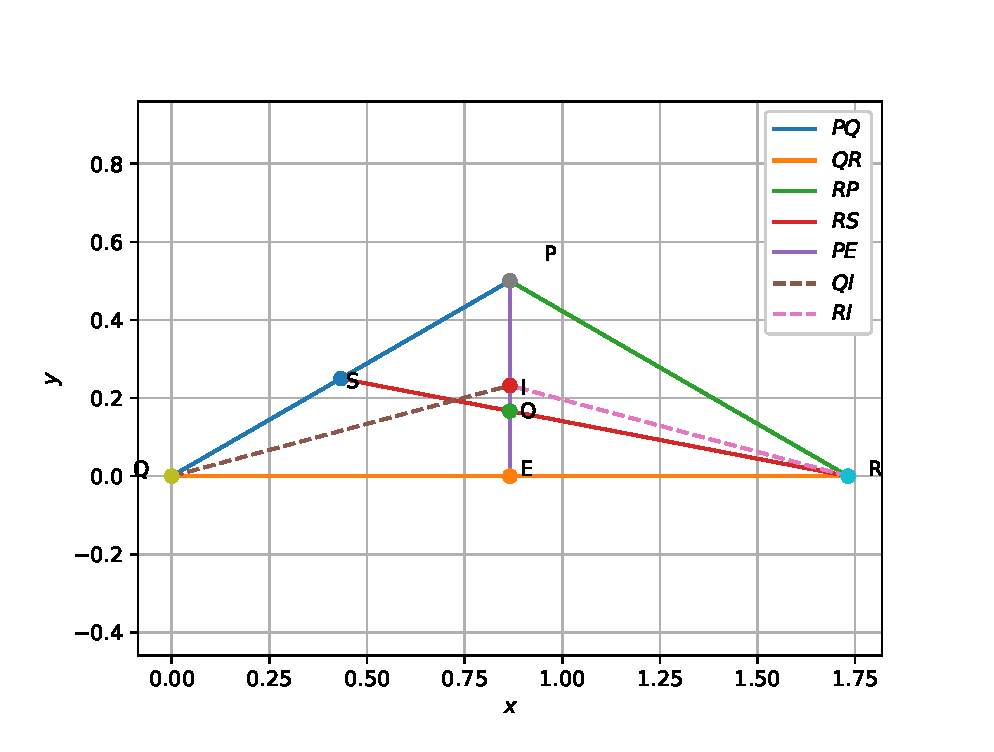
\includegraphics[width=\columnwidth]{./figs/2019_8.eps}
\caption{}
\label{fig:2019_8}
\end{figure}
%
Using the cosine formula, 
\begin{align}
RS &= \sqrt{q^2+\brak{\frac{r}{2}}^2-qr\cos P}
\\
&= \sqrt{1+\frac{1}{4}+\frac{1}{2}} = \sqrt{\frac{7}{2}}
\end{align}
\item Find $OE$.
\\
\solution 
Using Baudhayana's theorem,
\begin{align}
OE  &= \sqrt{OR^2 - ER^2}
\\
&= \sqrt{\brak{\frac{2RS}{3}}^2 - \brak{\frac{p}{2}}^2} 
\\
&= \sqrt{\frac{7}{9}-\frac{3}{4}} = \frac{1 }{6}
\end{align}
%
\item Find the area of $\triangle SOE$
\\
\solution
$\because$ $PE$ and $RS$ are medians, 
\begin{align}
\text{ar}\brak{\triangle SOE }&= \frac{1}{4}\text{ar}\brak{\triangle POR},
\\
\text{ar}\brak{\triangle POR }&=  \frac{2}{3}\text{ar}\brak{\triangle PER},
\\
\text{ar}\brak{\triangle PER }&=  \frac{1}{2}\text{ar}\brak{\triangle PQR},
\\
\implies \text{ar}\brak{\triangle SOE} &= \frac{1}{12}\text{ar}\brak{\triangle PQR}
&= \frac{\sqrt{3}}{24}
\end{align}

\item Find the radius of the incircle of $\triangle PQR $.
%
\\
\solution
I is the incentre in Fig. \ref{fig:2019_8}.  The radius of the incircle is 
\begin{align}
\frac{p}{2\cos\frac{Q}{2}} &= \frac{p}{\sqrt{2\brak{1+\cos Q}}}
\\ &= \sqrt{\frac{3}{1+\sqrt{3}}}
\end{align}
%
\item Repeat all the above exercises using vector algebra and plot Fig. \ref{fig:2019_8}.
\end{enumerate}
%
\section{Coordinate Geometry}
Let the ellipse $E_1, n = 1, 2,  \dots$ have the equation 
\begin{align}
\vec{x}^T\vec{D}\vec{x} = 1,
\end{align}
%
where 
\begin{align}
\vec{D} = \myvec{\frac{1}{a^2} & 0 \\ 0 & \frac{1}{b^2}} 
\end{align}
\begin{enumerate}[label=\thesection.\arabic*
,ref=\thesection.\theenumi]
\item Let the largest rectangle inside $E_1$  with sides parallel to the axebe be $R_1$.
Show that the coordinates of the $R_1$ have the form
\begin{align}
 \myvec{\pm p_1 \\ \pm p_2}
\end{align}
\solution Let $R_1$ be the rectangle $PQRS$, where $PQ \parallel RS \parallel x-axis, QR \parallel PS \parallel y-axis $. Their corresponding equations are 
\begin{align}
\label{eq:9_pq}
PQ: \vec{x} = \vec{P} +  \lambda_1 \vec{m}_1
\\
\label{eq:9_ps}
PS: \vec{x} = \vec{P} +  \lambda_2 \vec{m}_2
\\
\label{eq:9_qr}
QR: \vec{x} = \vec{Q} +  \lambda_3 \vec{m}_2
%RS: \vec{x} = \vec{S} +  \lambda_2 \vec{m}_1
\end{align}
%
where 
\begin{align}
\vec{m}_1=\myvec{1\\  0},
\vec{m}_2=\myvec{0\\  1}
\end{align}
The intersection of $PQ$ with $E_1$ is
\begin{align}
\sbrak{\vec{P} +  \lambda_1 \vec{m}_1}^T\vec{D}\sbrak{\vec{P} +  \lambda_1 \vec{m}_1} &= 1
\nonumber \\
\implies \lambda_1^2 \norm{\vec{m}_1}^2 + 2\lambda_1 \vec{m}_1^T\vec{P}+\vec{P}^T\vec{D}\vec{P} -1 & = 0
\nonumber 
\end{align}
\begin{align}
\because \vec{P} \in E_1, \norm{\vec{m}_1}^2  = 1, \vec{P}^T\vec{D}\vec{P} -1 &= 0
\nonumber \\
\implies \lambda_1 = 0, -2\vec{m}_1^T\vec{P}
\end{align}
%
Thus,
\begin{align}
\vec{Q} &= \vec{P}   -2\vec{m}_1^T\vec{P} \vec{m}_1
\nonumber \\
&= \myvec{-p_1 \\ p_2}
\end{align}
%
Similarly, 
\begin{align}
\vec{S} &= \vec{P}   -2\vec{m}_2^T\vec{P} \vec{m}_2
\nonumber \\
&= \myvec{p_1 \\ -p_2}
\end{align}
%
and 
\begin{align}
\vec{R} &= \vec{Q}   -2\vec{m}_2^T\vec{Q} \vec{m}_2
\nonumber \\
&= \myvec{-p_1 \\ -p_2}
\end{align}
\item Find an expression for the square of the area of $R_1$.
\\
\solution 
\begin{align}
\because \frac{p_1^2}{a^2}+\frac{p_2^2}{b^2} = 1,
\nonumber \\
p_2 = b \sqrt{1 - \frac{p_1^2}{a^2}}.
\label{eq:9_p2}
\end{align}
%
Hence the desired expression is 
\begin{align}
\label{eq:9_f}
F = \brak{PQ\times QR}^2 = 16 p_1^2 p_2^2 = 16 p_1^2b^2 \brak{1 - \frac{p_1^2}{a^2}}.
\end{align}
%
\item Find $p_1$ that maximises $F$.
\\
\solution \eqref{eq:9_f} can be expressed as
\begin{align}
F &=  a^2b^2 \brak{16 a^2p_1^2 - 16p_1^4}
\nonumber \\
 &=  a^2b^2 \cbrak{a^4-\brak{a^2-4p_1^2}^2 }
\end{align}
%
Thus, $F$ is maximum when 
\begin{align}
\brak{a^2-4p_1^2}^2 &= 0
\nonumber \\
\implies p_1 = \pm \frac{a}{2}
\label{eq:9_p1sol}
\end{align}
\item Verify the above result graphically.
\item Find $p_2$.
\\
\solution From \eqref{eq:9_p2}
\begin{align}
 p_2 = \pm\frac{ \sqrt{3}}{2}b
\label{eq:9_p2sol}
\end{align}
%
\item Find $E_2$, the largest ellipse within $R_1$.
\solution From \eqref{eq:9_p1sol} and \eqref{eq:9_p2sol}, the  and semi-major/minor axes of $E_2$ are
\begin{align}
E_2: \brak{ \frac{a}{2},\frac{\sqrt{3}}{2}b}
\end{align}
%
\item find $E_n$ and $R_n$,
\\
\solution From \eqref{eq:9_p1sol} and \eqref{eq:9_p2sol}, the vertices of $R_n$ and semi-major/minor axes of $E_n$ are
\begin{align}
R_n: \cbrak{\pm \frac{a}{2^{n}},\pm\brak{\frac{\sqrt{3}}{2}}^nb}
\nonumber \\
E_n: \cbrak{ \frac{a}{2^{n-1}},\brak{\frac{\sqrt{3}}{2}}^{n-1}b}
\end{align}
In the following questions, $a=3,b=2$. Use a computer program.
\item Is the eccentricity $e_18=e_19$?
\item Verify if 
\begin{align}
\sum_{n=1}^{N}\brak{\text{Area of } R_n} < 24, 
\end{align}
for each positive integer $N$.
\item Is the length of the latus rectum of $E_9 = \frac{1}{6}$?
\item Is the distance of a focus from the centre in $E_9 = \frac{\sqrt{5}}{32}$?
\end{enumerate}

\section{Calculus: Differentiation}
Let 
{\small
\begin{align}
f(x) = 
\begin{cases}
x^5+5x^4+10x^3+10x^2+3x+1 & x < 0
\\
x^2-x+1 & 0 \le  x < 1
\\
\frac{2}{3}x^3-4x^2+7x-\frac{8}{3} & 1 \le x < 3
\\
\brak{x-2}\ln \brak{x-2}-x + \frac{10}{3} & x \ge 3
\end{cases}
\end{align}
}
\begin{enumerate}[label=\thesection.\arabic*
,ref=\thesection.\theenumi]
\item Is $f$ increasing in $\brak{-\infty, 0}$?	
\\
\solution 
\begin{align}
f^{\prime}(x) = 5x^4+20x^3+30x^2+20x+3 \quad  x < 0 &
\nonumber \\
\implies f^{\prime}(-1) = 5-20+30-20+3 =-2 < 0 &
\end{align}
%
Hence $f^{\prime}(x)$ is non-increasing.

\item Does $f^{\prime}$ have a local maximum at $x = 1$?
\\
\solution 
\begin{align}
\label{eq:cont_diff}
f^{\prime}(x)=
\begin{cases}
  2x-1 > 0, &  \frac{1}{2} < x < 1,
\\
2\brak{x-2}^2 -1 < 0 & 1 \le x < 3
\end{cases}
\end{align}
Hence, $f$ is increasing in $\brak{\frac{1}{2},1}$ and decreasing between $\brak{1, 3} \implies f$ has a local maximum at $x=1$
\item Show that $f^{\prime}$ is differentiable at $x = 1$.
\\
\solution Since
\begin{align}
f^{\prime}(1-)=
f^{\prime}(1)=1,
\end{align}
$f$ is differentiable at $x = 1$.
\item Is $f$ onto?
\item Sketch $f(x)$ in Python to verify your answeres.

\end{enumerate}

\section{Calculus: Differential Equations}
$\Gamma$ is a curve in the first qudrant and 
\begin{align}
\vec{R} = \myvec{1 \\ 0}
\end{align}
%
lies on it.  The tangent to $\Gamma$ at $\vec{P}$ intersects the $y-$axis at $\vec{Y}_P$. The line segment $PY_P = 1$. 
%
\begin{enumerate}[label=\thesection.\arabic*
,ref=\thesection.\theenumi]
\item Find the differential equation of $\Gamma$.
\\
\solution Let 
\begin{align}
\vec{P}=\myvec{x \\ y},
\vec{Y}_P=\myvec{0 \\ c}.
\end{align}
%
Then using the equation of a line, 
\begin{align}
\vec{Y}_P=\vec{P} + \lambda \vec{m},
\end{align}
%
where 
\begin{align}
\vec{m}=\myvec{1\\ y^{\prime}}.
\end{align}
%
Thus, 
\begin{align}
\myvec{0 \\ c}&=\myvec{x \\ y} + \lambda \myvec{1\\ y^{\prime}}
\\
\implies \lambda &= -x.
\end{align}
\begin{align}
\because PY_P =  \norm{\vec{P}-\vec{Y}_P} &= \abs{\lambda} \norm{\vec{m}} = 1,
\\
x^2\brak{1 + \brak{y^{\prime}}^2} &= 1
\\
\implies xy^{\prime}  \pm \sqrt{1-x^2} &= 0
\label{eq:diffeq}
\end{align}
%
\item Find the equation of $\Gamma$.
\\
\solution From \eqref{eq:diffeq},
\begin{align}
dy &=   \pm \frac{\sqrt{1-x^2}}{ x}\,dx
\\
\implies \int \, dy &=   \pm \int\frac{\sqrt{1-x^2}}{ x}\,dx
%\label{eq:diffeq}
\end{align}
%
Letting 
\begin{align}
z = \sqrt{1-x^2},
dz &= -\frac{x}{\sqrt{1-x^2}}\, dx
\nonumber \\
\implies \int\frac{\sqrt{1-x^2}}{ x}\,dx &= -\int\frac{z^2}{ 1-z^2}\,dz
\nonumber \\
 &= \int\,dz-\int\frac{1}{ 1-z^2}\,dz
\nonumber \\
 &= z + \frac{1}{2}\ln \frac{1-z}{1+z} + C
\end{align}
Thus, 
\begin{align}
y = \pm \brak{\sqrt{1-x^2} + \frac{1}{2}\ln \frac{1-\sqrt{1-x^2}}{1+\sqrt{1-x^2}}} 
\end{align}
since $C=0$ after substituting $x=0, y = 1$.
\item Verify your result through a python sketch.
\end{enumerate}

\section{Linear Algebra: Orthogonality}
\begin{enumerate}[label=\thesection.\arabic*
,ref=\thesection.\theenumi]

\item Let
\begin{align}
L_1: \quad \vec{x} &= \myvec{1 \\ 0 \\ 0} + \lambda_1 \myvec{-1 \\ 2 \\ 2}
\\
L_2: \quad \vec{x} &=  \lambda_1 \myvec{2 \\-1 \\ 2}
\end{align}
%
Given that  $L_3 \perp L_1, L_3 \perp L_2$, find $L_3$.
\\
\solution Let 
\begin{align}
L_3: \quad \vec{x} &= \vec{c}+ \lambda \vec{m}_3
\end{align}
% 
Then
\begin{align}
\myvec{-1 & 2 & 2
\\
2 &-1 & 2}\vec{m}_3 = \vec{0}
\end{align}
%
Row reducing the coefficient matrix,
\begin{align}
\myvec{-1 & 2 & 2
\\
2 &-1 & 2} &\leftrightarrow 
\myvec{1 & -2 & -2
\\
0 &1 & 2} 
\\
\leftrightarrow 
\myvec{1 & 0 & 2
\\
0 &1 & 2} 
& \implies \vec{m}_3 = \myvec{2 \\ 2 \\ -1}
\end{align}
%
Also, $L_1\perp L_2$, but $L_1 \cup L_2 = \phi$. The given information can be summarized as
\begin{align}
\label{eq:12-given1}
L_1: \quad \vec{x} &= \vec{c}_1 + \lambda_1 \vec{m}_1
\\
L_2: \quad \vec{x} &=  \lambda_2 \vec{m}_2
\\
L_3: \quad \vec{x} &= \vec{c}_3 + \lambda \vec{m}_3
\label{eq:12-given3}
\end{align}
%
where
\begin{align}
\label{eq:12-given12}
\vec{c}_1 = \myvec{1 \\ 0 \\ 0}, \vec{m}_1=  \myvec{-1 \\ 2 \\ 2},
\vec{m}_2 = \myvec{2 \\-1 \\ 2}
\end{align}
The objective is to find $\vec{c}_3$.  Since $L_1 \cup L_3 \ne \phi, L_2 \cup L_3 \ne \phi$, from \eqref{eq:12-given1}-\eqref{eq:12-given3},
\begin{align}
\label{eq:12-isect13}
\vec{c}_1 + \lambda_1 \vec{m}_1 &= \vec{c}_3 + \lambda_3 \vec{m}_3
\\
  \lambda_2 \vec{m}_2 &= \vec{c}_3 + \lambda_4 \vec{m}_3
\label{eq:12-isect23}
\end{align}
%
Using the fact that $L_1\perp L_2\perp L_3$, \eqref{eq:12-isect13}-\eqref{eq:12-isect23} can be expressed as
\begin{align}
%\label{eq:12-isect13}
\vec{m}_1^T\vec{c}_1 + \lambda_1 \norm{\vec{m}}_1^2 &= \vec{m}_1^T\vec{c}_3 
\\
\vec{m}_2^T\vec{c}_1  &= \vec{m}_2^T\vec{c}_3 
\\
\vec{m}_3^T\vec{c}_1  &= \vec{m}_3^T\vec{c}_3 + \lambda_3 \norm{\vec{m}_3}^2
\\
0 &= \vec{m}_1^T\vec{c}_3 
\\
  \lambda_2 \norm{\vec{m}_2}^2 &= \vec{m}_2^T\vec{c}_3 
\\
0 &= \vec{m}_3^T\vec{c}_3  + \lambda_4 \norm{\vec{m}_3}^2
%\label{eq:12-isect23}
\end{align}
%
Simplifying the above, 
\begin{align}
 \lambda_1  &= -\frac{\vec{m}_1^T\vec{c}_1}{\norm{\vec{m}}_1^2} = \frac{1}{9}
\\
 \lambda_2  &= \frac{\vec{m}_2^T\vec{c}_1}{\norm{\vec{m}}_2^2} =\frac{2}{9}
\end{align}
%
Substituting in \eqref{eq:12-isect13} and \eqref{eq:12-isect23},
\begin{align}
L_3: \quad \vec{x} &= \frac{2}{9}\myvec{4 \\ 1 \\ 1} + \lambda_3\myvec{2 \\ 2 \\ -1} \text{ or}
\\
L_3: \quad \vec{x} &= \frac{2}{9}\myvec{2 \\-1 \\ 2} + \lambda_3\myvec{2 \\ 2 \\ -1}
\end{align}
%
The key concept in this question is that orthogonality of $L_1$ and $L_2$ doesnot mean that they intersect.  They are skew lines.
\end{enumerate}
%
\section{Linear Algebra: Eigenvalue and Eigenvector}
\begin{enumerate}[label=\thesection.\arabic*
,ref=\thesection.\theenumi]
\item Obtain the  $3 \times 3$ matrices $\cbrak{\vec{P}_k}_{k=1}^{6}$ from the vectors
\begin{align}
\vec{v}_1 = \myvec{0 & 0 & 1}
\\
\vec{v}_2 = \myvec{0 & 1 & 0}
\\
\vec{v}_3 = \myvec{1 & 0 & 0}
\end{align}
%
and  let 
\begin{align}
\vec{X} = \sum_{k=1}^{6}\vec{P}_k\myvec{2 & 1 & 3 \\ 1 & 0 & 2 \\ 3 & 2 & 1}\vec{P}_k^T
\end{align}
%
Verify if 
\begin{enumerate}
\item $\lambda = 30$ is an eigenvalue of $\vec{X}$ and  $\vec{x} = \myvec{1 & 1 & 1}^T$ the corresponding eigenvector.
\item $\vec{X}$ is symmetric.
\item $\text{tr}\brak{\vec{X}} = 18$.
\item $\vec{X}-30\vec{I}$ is invertible.
\end{enumerate}
\item Let 
\begin{align}
\vec{P} = \myvec{1 & 1 & 1 \\ 0 & 2 & 2 \\ 0 & 0 & 3}, 
\vec{Q} = \myvec{2 & x & x \\ 0 & 4 & 0 \\ x & x & 6}
\end{align}
Verify if 
\begin{enumerate}
\item $PQ=QP$ for some $x$.
\item 
$
\det{R}= 
\det\myvec{2 & x & x \\ 0 & 4 & 0 \\ x & x & 5}
$ 
for all $x$.
\item for $x= 0$, if $\vec{R}\myvec{1 \\ a \\ b} = 6\myvec{1 \\ a \\ b}$, then $a+b = 5$. {\em Use property of eigenvector}.
\item For $x = 1$, there exists a  vector $\vec{y}$ for whcih $\vec{R}\vec{y} = \vec{0}$. This implies that the null space of $\vec{R}$ is nonempty. Also, $\vec{R}$ is noninvertible, $\det(R)=0$ and has a 0 eigenvalue.

\end{enumerate}
\item
\item
\item
\item
\item
\item Let
\begin{align}
\label{eq:qp2-8-l_1}
L_1: \quad \vec{r} = \lambda_1 \myvec{1\\0\\0}
\\
\label{eq:qp2-8-l_2}
L_2: \quad \vec{r} = \myvec{0\\0\\1}+\lambda_2 \myvec{0\\1\\0}
\\
L_3: \quad \vec{r} =  \myvec{1\\1\\0}+\lambda_3 \myvec{0\\0\\1}
\label{eq:qp2-8-l_3}
\end{align}
%
Let $\vec{P}\in L_1, \vec{Q}\in L_2, \vec{R}\in L_3$. Verify if  $\vec{Q}$ can be 
\begin{enumerate}
\item $\myvec{0\\-\frac{1}{2} \\ 1}$
\item $\myvec{0\\ 0\\1}$
\item $\myvec{0\\ \frac{1}{2} \\1}$
\item $\myvec{0\\1 \\1}$
\end{enumerate}
given that   $\vec{P},\vec{Q},\vec{R}$ are collinear.
\\
\solution 
%Let
%\begin{align}
%\label{eq:qp2-8-l_4}
%L_4: \quad \vec{r} = \vec{c}_4+\lambda_4 \vec{m}_4
%\end{align}
%%
%be the line passing through $L_1,L_2,L_3$ at $\vec{P},\vec{Q},\vec{R}$ respectively. 
If $\vec{P},\vec{Q},\vec{R}$ are collinear,
\begin{align}
\frac{PQ}{QR} &= k,
\\
\brak{k+1}\vec{Q} &= k\vec{P}+ \vec{R},
\label{eq:qp2-8-coll}
\end{align}
From \eqref{eq:qp2-8-l_1}, \eqref{eq:qp2-8-l_2} and \eqref{eq:qp2-8-l_3},
\begin{multline}
k \lambda_1 \myvec{1\\0\\0}
+\myvec{1\\1\\0}+\lambda_3 \myvec{0\\0\\1}
\\
=
\brak{k+1} \myvec{0\\0\\1}+\brak{k+1}\lambda_2 \myvec{0\\1\\0}
\end{multline}
%
which can be expressed as
\begin{align}
\myvec{k & 0 & 0
\\
0 & -\brak{k+1} & 0
\\
0 & 0 & 1
}
\myvec{\lambda_1\\\lambda_2\\ \lambda_3}
=\myvec{-1 \\ -1 \\ k+1}
\end{align}
%
Thus,
\begin{align}
\vec{Q} = \myvec{0 \\\frac{1}{k+1} \\1}
\end{align}
\end{enumerate}
\end{document}


